\documentclass[footinclude=false,11pt,DIV11]{scrartcl}

% Wenzel's standard prelude
% ----- 8< ----- 8< ------

\usepackage[english]{babel}
\usepackage[T1]{fontenc}
\usepackage[utf8]{inputenc}
\usepackage{graphicx}
\usepackage{amsmath}
\usepackage{mathtools}
\usepackage{array}
\usepackage{booktabs}
\usepackage{tabularx}
\usepackage{color}
\usepackage{colortbl}
\usepackage{listings}
\usepackage{enumerate}
\usepackage{upquote}
\usepackage[absolute]{textpos} % Manual placement of certain things
\usepackage{ragged2e} % Ragged-right columns with hyphenation
\usepackage{nicefrac}
\usepackage{macros}
\usepackage[format=hang,font=small,labelfont=bf]{caption}
\usepackage[expansion=false, babel=true]{microtype}
\usepackage{subfig}
\usepackage{ifthen}
\usepackage{longtable}
\usepackage{wrapfig}
\usepackage{footnote} % savenotes environment

% Make sure that ligatures remain searchable in the PDF
\input glyphtounicode
\pdfgentounicode=1

\IfFileExists{MinionPro.sty}
   {\usepackage[opticals,fullfamily,lf]{MinionPro}}
   {\usepackage{charter}\message{Package MinionPro.sty was not found. Reverting to charter.}}

\setcounter{secnumdepth}{3}
\setcounter{tocdepth}{3}

\newcommand{\MitsubaVersion}{0.4.2}
\newcommand{\MitsubaYear}{2012}

\typearea[current]{last}
\raggedbottom
\renewcommand*\ttdefault{txtt}

\usepackage{scrpage2}
\ofoot[]{}
\cfoot[]{}
\automark[subsection]{section}
\ihead{\sc\leftmark}
\ohead{\sc\rightmark}
\chead{}
\setheadsepline{.2pt}
\setkomafont{pagenumber}{\normalfont}
\addtokomafont{sectioning}{\color{myblue}\rmfamily}
\addtokomafont{descriptionlabel}{\rmfamily}
\pagestyle{scrheadings}

\usepackage[
	bookmarks,
	bookmarksnumbered,
	colorlinks,
	plainpages=false,
	pdfpagelabels,
	hypertexnames=false,
	linkcolor=myblue,
	urlcolor=myblue,
	citecolor=myblue,
	pdfpagelabels,
	pdftitle={Mitsuba \MitsubaVersion\, Documentation},
	pdfauthor={Wenzel Jakob},
	pdfstartview=FitH
]{hyperref}

\definecolor{myblue}{rgb}{0,.1,.6}
\definecolor{myred}{rgb}{0.63,.16,.16}
\definecolor{lstshade}{gray}{0.95}
\definecolor{lstframe}{gray}{0.80}
\definecolor{lstcomment}{gray}{0.5}
\definecolor{lstattrib}{rgb}{0,0.34,0}
\definecolor{remark}{rgb}{1.0, 0.9, 0.9}
\definecolor{remarkframe}{rgb}{1.0, 0.7, 0.7}

% Listings settings
\lstset{
	basicstyle = \small\ttfamily\raggedright,
	commentstyle=\color{lstcomment}\itshape,
	stringstyle=\color{lstattrib},
	mathescape = true,
	frame = lrtb,
	backgroundcolor = \color{lstshade},
	rulecolor = \color{lstframe},
	tabsize = 4,
	columns = flexible,
	keepspaces,
	belowskip = \smallskipamount,
	framerule = .7pt,
	breaklines = true,
	showstringspaces = false,
	keywordstyle = \bfseries,
	captionpos = b,
	upquote = true
}

\lstdefinelanguage{xml} {
	sensitive=true,
	morecomment=[s][\color{lstcomment}\itshape]{<!--}{-->},
	morecomment=[s][\color{lstcomment}]{<?}{?>},
	string=[b]", stringstyle=\color{lstattrib},
	keywords= [1] {
		shape,bsdf,scene,texture,phase,integer,float,
		string,transform,ref,rgb,srgb,spectrum,blackbody,
		medium,film,sampler,integrator,emitter,sensor,
		translate,rotate,scale,lookat,point,vector,matrix,
		include,fscat,volume,alias,rfilter,boolean,
		subsurface,animation
	},
}


% Set up textpos
\TPGrid{68}{108}

% Thick frames for images
\setlength\fboxsep{0pt}
\setlength\fboxrule{1.5pt}

% Less vertical spacing for \figure[h] floats
\setlength{\intextsep}{3pt}

\lstnewenvironment{shell}[1][]{\lstset{#1}}
	{}
\lstnewenvironment{cpp}[1][]{\lstset{language=c++, #1}}
	{}
\lstnewenvironment{python}[1][]{\lstset{language=Python, #1}}
	{}
\lstnewenvironment{xml}[1][]{\lstset{language=xml, #1}}
	{}
\lstnewenvironment{console}[1][]{\lstset{basicstyle=\footnotesize\ttfamily, float, #1}}
	{}

% ----- 8< ----- 8< ------

\title{
	\vspace{3cm}
	
\includegraphics[width=4cm]{images/logo_plain.pdf}\\\vspace{1.5cm}
	\Huge
	Mitsuba Documentation\\\vspace{4mm}
	\LARGE Version \MitsubaVersion
	\vspace{5mm}
}
\author{Wenzel Jakob}
\date{\today}

\begin{document}
\maketitle
\clearpage
\ofoot[\pagemark]{\pagemark}

\tableofcontents

\part{Using Mitsuba}
\textbf{Disclaimer:} This is manual documents the usage, file format, and
internal design of the Mitsuba rendering system. It is currently a work
in progress, hence some parts may still be incomplete or missing.

\section{About Mitsuba}
Mitsuba is a research-oriented rendering system in the style of PBRT
(\url{www.pbrt.org}), from which it derives much inspiration.
It is written in portable C++, implements unbiased as well
as biased techniques, and contains heavy optimizations targeted
towards current CPU architectures.
Mitsuba is extremely modular: it consists of a small set of core libraries
and over 100 different plugins that implement functionality ranging
from materials and light sources to complete rendering algorithms.

In comparison to other open source renderers, Mitsuba places a strong
emphasis on experimental rendering techniques, such as path-based
formulations of Metropolis Light Transport and volumetric
modeling approaches. Thus, it may be of genuine interest to those who
would like to experiment with such techniques that haven't yet found
their way into mainstream renderers, and it also provides a solid
foundation for research in this domain.

Other design considerations are:

\parheader{Performance:}
Mitsuba provides optimized implementations of the most commonly
used rendering algorithms. By virtue of running on a shared foundation, comparisons between them can
better highlight the merits and limitations of different approaches. This is in contrast to, say,
comparing two completely different rendering products, where technical information on the underlying
implementation is often intentionally not provided.

\parheader{Robustness:}
In many cases, physically-based rendering packages force the user to model scenes with the underlying
algorithm (specifically: its convergence behavior) in mind. For instance, glass windows are routinely
replaced with light portals, photons must be manually guided to the relevant parts of a scene, and
interactions with complex materials are taboo, since they cannot be importance sampled exactly.
One focus of Mitsuba will be to develop path-space light transport algorithms, which handle such
cases more gracefully.

\parheader{Scalability:} Mitsuba instances can be merged into large clusters, which transparently distribute and
jointly execute tasks assigned to them using only node-to-node communcation. It has successfully
scaled to large-scale renderings that involved more than 1000 cores working on a single image.
Most algorithms in Mitsuba  are written using a generic parallelization layer, which can tap
into this cluster-wide parallelism. The principle is that if any component of the renderer produces
work that takes longer than a second or so, it at least ought to use all of the processing power
it can get.

The renderer also tries to be very conservative in its use of memory, which allows it to handle
large scenes (>30 million triangles) and multi-gigabyte heterogeneous volumes on consumer hardware.

\parheader{Realism and accuracy:} Mitsuba comes with a large repository of physically-based
reflectance models for surfaces and participating media. These implementations
are designed so that they can be used to build complex shader networks, while
providing enough flexibility to be compatible with a wide range of different
rendering techniques, including path tracing, photon mapping, hardware-accelerated rendering
and bidirectional methods.

The unbiased path tracers in Mitsuba are battle-proven and produce
reference-quality results that can be used for predictive rendering, and to verify
implementations of other rendering methods.

\parheader{Usability:}
Mitsuba comes with a graphical user interface to interactively explore scenes. Once a suitable
viewpoint has been found, it is straightforward to perform renderings using any of the
implemented rendering techniques, while tweaking their parameters to find the most suitable
settings. Experimental integration into Blender 2.5 is also available.

\section{Limitations}
Mitsuba can be used to solve many interesting light transport problems.
However, there are some inherent limitations of the system that users should be aware of:
\begin{enumerate}[(i)]
\item \textbf{Wave Optics}: Mitsuba is fundamentally based on the geometric optics toolbox,
which means that it generally does not simulate phenomena that arise due to
the wave properties of light (diffraction, for instance).
\item \textbf{Polarization}: Mitsuba does not account for polarization. In
other words, light is always assumed to be randomly polarized. This can be a problem for
some predictive rendering applications.
\item \textbf{Numerical accuracy}: The accuracy of any result produced with this
system is constrained by the underlying floating point computations.

For instance, an intricate scene that can be rendered without problems,
may produce the wrong answer when all objects are translated away from the
origin by a large distance, since floating point numbers are spaced less densely at the
new position.  To avoid these sorts of pitfalls, it is good to have a basic
understanding of the IEEE-754 standard.
\end{enumerate}

\section{License}
Mitsuba is free software and can be redistributed and modified under the terms of the GNU General
Public License (Version 3) as provided by the Free Software Foundation.

\remarks{
	\item Being a ``viral'' license, the GPL automatically applies to all
	derivative work. Amongst other things, this means that without express
	permission, Mitsuba's source code is \emph{off-limits} to companies that
	develop rendering software not distributed under a compatible license.
}

\section{Compiling the renderer}
To compile Mitsuba, you will need a recent C++ compiler (e.g. GCC 4.1+ or 
Visual Studio 2005+) and some additional libraries, which Mitsuba uses internally. 
Builds on all three supported platforms are done using a unified system
based on SCons (\url{http://www.scons.org}), a flexible python-based 
software construction tool. There are some minor differences between operating systems though: for
more details, please refer to one of the next sections depending on which one you use.

\subsection{Common steps}
To get started, you will need to download a recent version of Mitsuba: make sure that you have the Mercurial (\url{http://mercurial.selenic.com/})
versioning system installed and enter the following at the command prompt:
\begin{shell}
$\texttt{\$}$ hg clone https://www.mitsuba-renderer.org/hg/mitsuba
\end{shell}
On Windows, you can instead use the more convenient TortoiseHG shell extension (\url{http://tortoisehg.bitbucket.org/}) 
to do this directly from the Explorer.

Common to all platforms is that a build configuration file must be chosen: amongst the
following, please copy the best matching file into a new file to the root of the Mitsuba
directory and rename it into \code{config.py}.
\begin{shell}
config/config-linux.py  
config/config-darwin-x86_64.py  
config/config-darwin-x86.py  
config/config-darwin-universal.py  
config/config-msvc2005-win32.py  
config/config-msvc2005-win64.py
\end{shell}

Some minor adjustments may have to be made to this file based on your configuration. 
You may also set adjust certain compilation flags here:
\begin{description}
\item[\texttt{MTS\_DEBUG}] Enable assertions etc. Usually a good idea.
\item[\texttt{SINGLE\_PRECISION}] Do all computation in single precision. This is usually sufficient.
\item[\texttt{DOUBLE\_PRECISION}] Do all computation in double precision. Incompatible with
\texttt{MTS\_SSE}, \texttt{MTS\_HAS\_COHERENT\_RT}, and \texttt{MTS\_DEBUG\_FP}.
\item[\texttt{MTS\_SSE}]Activate optimized SSE routines.
\item[\texttt{MTS\_HAS\_COHERENT\_RT}]Include coherent ray tracing support (depends on \texttt{MTS\_SSE}).
\item[\texttt{MTS\_DEBUG\_FP}]Generated NaNs will cause floating point exceptions, which can be caught in a debugger. Warning: This is slow!
\end{description}
All default configurations use the flags \code{MTS\_DEBUG}, \code{SINGLE\_PRECISION}, \code{MTS\_SSE}, \code{MTS\_HAS\_COHERENT\_RT}.
Initially, it is a good idea to just leave the configuration the way it is.

\subsection{Building on Ubuntu Linux}
You'll first need to install a number of dependencies. It is assumed here
that you are using Ubuntu Linux, hence some of the package may be named differently if you are 
using another distribution.

First, run
\begin{shell}
$\text{\$}$ apt-get install build-essential scons qt4-dev-tools scons libpng12-dev libjpeg62-dev libilmbase-dev libopenexr-dev libxerces-c2-dev libboost-dev libglewmx1.5-dev libxxf86vm-dev libboost-system-dev libboost-filesystem-dev
\end{shell}
To get COLLADA support, you will also need to install the \texttt{collada-dom} packages or build them from scratch. Here, we install the \code{x86\_64} binaries and development headers included with Mitsuba:
\begin{shell}
$\text{\$}$ dpkg --install tools/linux/collada-dom2.2_2.2-1_amd64.deb tools/linux/collada-dom-dev_2.2-1_amd64.deb
\end{shell}
Afterwards, simply run
\begin{shell}
$\text{\$}$ scons
\end{shell}
inside the Mitsuba directory. In the case that you have multiple processors, you might want to parallelize the build by appending \code{-j }\emph{core count} to the command.
If all goes well, SCons should finish successfully within a few minutes:
\begin{shell}
scons: $\texttt{done}$ building targets.
\end{shell}
To be able to run the renderer from the command line, you will also have to import it into your path:
\begin{shell}
$\text{\$}$ . setpath.sh
\end{shell}
(note the period at the beginning -- this assumes that you are using \code{bash}).

\subsection{Building on Fedora Core}
You'll first need to install a number of dependencies. It is assumed here
that you are using Fedora Core, hence some of the package may be named differently if you are 
using another distribution.

First, run
\begin{shell}
$\text{\$}$ yum install mercurial gcc-c++ boost-devel qt4-devel OpenEXR-devel xerces-c-devel
\end{shell}
You will also need the \texttt{glew-mx} and \texttt{collada-dom} packages, which are not included in the Fedora package repository. You can grab source and \texttt{i386} binary \texttt{RPM} files here: \texttt{http://www.mitsuba-renderer.org/release}.
Afterwards, simply run
\begin{shell}
$\text{\$}$ scons
\end{shell}
inside the Mitsuba directory. In the case that you have multiple processors, you might want to parallelize the build by appending \code{-j }\emph{core count} to the command.
If all goes well, SCons should finish successfully within a few minutes:
\begin{shell}
scons: $\texttt{done}$ building targets.
\end{shell}
To be able to run the renderer from the command line, you will also have to import it into your path:
\begin{shell}
$\text{\$}$ . setpath.sh
\end{shell}
(note the period at the beginning -- this assumes that you are using \code{bash}).


\subsection{Building on Windows}
This section assumes that Visual Studio 2008 is installed, but the instructions should work equally well with other versions.
On the Windows platform, Mitsuba already includes most of the dependencies in precompiled form.
You will still need to set up a few things though: first, you need to install Python 
(\url{www.python.org}) and SCons (\url{http://www.scons.org}) and ensure that they are contained
in the \code{\%PATH\%} environment variable so that entering \code{scons} on the command prompt
(\code{cmd.exe}) launches the build system (it will complain about not finding a project file though).
\begin{shell}
C:\Users\Wenzel>scons
scons: ** No SConstruct file found.
\end{shell}
\emph{Note: }On some setups, the SCons installer generates a warning about not finding Python in the registry. In this case, you can instead run \code{python setup.py install} within the source release of SCons.
Next, install Qt (\url{http://qt.nokia.com/downloads/windows-cpp-vs2008} -- you should get the release for Visual Studio 2008). Again, you need to make sure that the 
Qt utilities are reachable through the \code{\%PATH\%} environment variable so that you can for example launch \code{moc.exe} from the command line.

Because the official release of Qt currently only contains 32-bit binaries, you will accordingly have to 
build Mitsuba in 32-bit mode (i.e. you should use the configuration file \code{config-msvc2005-win32.py}). If you would rather like compile it in 64-bit mode, you have to create
your own 64-bit Qt binaries.

Having installed these dependencies, run the ``Visual Studio 2008 Command 
Prompt'' from the Start Menu (pick the \code{x86} version if you have the choice beetween \code{x86} and \code{x64}). Afterwards,
navigate to the Mitsuba directory and run \code{scons}. 
In the case that you have multiple processors, you might want to parallelize the build by appending \code{-j }\emph{core count} to the \code{scons} command.

If all goes well, the build process will finish successfully after a few
minutes. In comparison to the other platforms, you don't have to run the \code{setpath.sh} script at this point. 
All binaries are now located in the \code{dist} directory, and they should be executed directly from there.

\subsection{Building on Mac OS X}
On Mac OS X, you will need to install both scons (\code{www.scons.org}) and 
a recent release of XCode. You will also need to get Qt 4.7.0 Beta 2 or a newer version.
As of this writing, 4.7.0 Beta 2 is still the most recent release and can be found here: \url{http://qt.nokia.com/developer/qt-qtcreator-prerelease#download}
--- make sure that you get the normal Cocoa release (i.e. \emph{not} the one based on Carbon). All of the
other dependencies are already included in precompiled form.

Now open a Terminal and run
\begin{shell}
$\text{\$}$ scons
\end{shell}
inside the Mitsuba directory. In the case that you have multiple processors, you might want to parallelize the build by appending \code{-j }\emph{core count} to the command.
If all goes well, SCons should finish successfully within a few minutes:
\begin{shell}
scons: $\texttt{done}$ building targets.
\end{shell}
To be able to run the renderer from the command line, you will have to import it into your path:
\begin{shell}
$\text{\$}$ . setpath.sh
\end{shell}
(note the period at the beginning -- this assumes that you are using \code{bash}).

\section{Basic usage}
\label{sec:basics}
The rendering functionality of Mitsuba can be accessed through
a command line interface and an interactive Qt-based frontend. This section
provides some basic instructions on how to use them.
\subsection{Interactive frontend}
To launch the interactive frontend, run \code{Mitsuba.app} on MacOS, 
\code{mtsgui.exe} on Windows, and \code{mtsgui} on Linux (after sourcing \code{setpath.sh}).
You can also drag and drop scene files onto the application icon or the running program to open them.
A quick video tutorial on using the GUI can be found here: \url{http://vimeo.com/13480342}.
\subsection{Command line interface}
\label{sec:mitsuba}
The \texttt{mitsuba} binary is an alternative non-interactive rendering 
frontend for command-line use and batch job operation.
To get a listing of the parameters it supports, run
the executable without parameters:
\begin{shell}
$\texttt{\$}$ mitsuba 
\end{shell}
\lstref{mitsuba-cli} shows the output resulting from this command. The most common
mode of operation is to render a single scene, which is provided as a parameter, e.g.
\begin{shell}
$\texttt{\$}$ mitsuba path-to/my-scene.xml
\end{shell}
It is also possible to connect to network render nodes, which essentially lets Mitsuba parallelize
over additional cores. To do this, pass a semicolon-separated list of machines to 
the \code{-c} parameter. 
\begin{shell}
$\texttt{\$}$ mitsuba -c machine1;machine2;... path-to/my-scene.xml
\end{shell}
There are two different ways in which you can access render nodes:
\begin{itemize}
\item\textbf{Direct}: Here, you create a direct connection to a running \code{mtssrv} instance on
another machine (\code{mtssrv} is the Mitsuba server process). From the the performance 
standpoint, this approach should always be preferred over the SSH method described below when there is 
a choice between them. There are some disadvantages though: first, you need to manually start
\code{mtssrv} on every machine you want to use. 

And perhaps more importantly: the direct communication
protocol makes no provisions for a malicious user on the remote side. It is too costly
to constantly check the communication stream for illegal data sequences, so Mitsuba simply doesn't do it.
The consequence of this is that you should only use the direct communication approach within
trusted networks.

For direct connections, you can specify the remote port as follows:
\begin{shell}
$\texttt{\$}$ mitsuba -c machine:1234 path-to/my-scene.xml
\end{shell}
When none is given, Mitsuba assumes that the server uses default port 7554. 
\item \textbf{SSH}: 
    This approach works as follows: The renderer creates a SSH connection 
	to the remote side, where it launches a Mitsuba worker instance.
	All subsequent communication then passes through the encrypted link. 
	This is completely secure but slower due to the encryption overhead.
	If you are rendering a complex scene, there is a good chance that it
	won't matter much since most time is spent doing computations rather than
	communicating

	Such an SSH link can be created simply by using a slightly different syntax:
\begin{shell}
$\texttt{\$}$ mitsuba -c username@machine path-to/my-scene.xml
\end{shell}
	The above line assumes that the remote home directory contains
	a Mitsuba source directory (with compiled binaries) named \code{mitsuba}.
	If that is not the case, you need to provide the path to such a directory manually, e.g:
\begin{shell}
$\texttt{\$}$ mitsuba -c username@machine:/opt/mitsuba path-to/my-scene.xml
\end{shell}
	For the SSH connection approach to work, you \emph{must} enable passwordless 
	authentication.
	Try opening a terminal window and running the command \code{ssh username@machine} 
	(replace with the details of your remote connection).
	If you are asked for a password, something is not set up correctly --- please see 
	\url{http://www.debian-administration.org/articles/152} for instructions.

	On Windows, the situation is a bit more difficult since there is no suitable SSH client by
	default. To get SSH connections to work, Mitsuba requires \code{plink.exe} (from PuTTY) to
	be on the path. For passwordless authentication with a Linux/OSX-based
	server, convert your private key to PuTTY's format using \code{puttygen.exe}.
	Afterwards, start \code{pageant.exe} to load and  authenticate the key. All 
	of these binaries are available from the PuTTY website, and there is also
	a copy in the \code{tools/windows/bin}
	directory in the Mitsuba repository.

	It is possible to mix the two approaches to access some machines directly and others
	over SSH.
\end{itemize}
When doing many network-based renders over the command line, it can become tedious to
specify the connections every time. They can alternatively be loaded from a text file
where each line contains a separate connection description as discussed previously:
\begin{shell}
$\texttt{\$}$ mitsuba -s servers.txt path-to/my-scene.xml
\end{shell}
where \code{servers.txt} e.g. contains
\begin{shell}
user1@machine1.domain.org:/opt/mitsuba
machine2.domain.org
machine3.domain.org:7346
\end{shell}
\subsubsection{Passing parameters}
Any attribute in the scene XML file can be parameterized from the
command line.
For instance, you can render a scene several times with different reflectance values
on a certain material by changing its description to something like 
\begin{xml}
<bsdf type="lambertian">
	<spectrum name="reflectance" value="$\texttt{\$}$reflectance"/>
</bsdf>
\end{xml}
and running Mitsuba as follows:
\begin{shell}
$\texttt{\$}$ mitsuba -Dreflectance=0.1 -o ref_0.1.exr scene.xml 
$\texttt{\$}$ mitsuba -Dreflectance=0.2 -o ref_0.2.exr scene.xml 
$\texttt{\$}$ mitsuba -Dreflectance=0.5 -o ref_0.5.exr scene.xml 
\end{shell}

\subsubsection{Writing partial images to disk}
When doing lengthy command line renders on Linux or OSX, it is possible 
to send a signal to the process using 
\begin{shell}	
$\texttt{\$}$ killall -HUP mitsuba
\end{shell}
This causes the renderer to write out the partially finished 
image, after which it continues rendering. This can sometimes be useful to 
check if everything is working correctly.

\subsubsection{Rendering an animation}
The command line interface is ideally suited for rendering large amounts of files in batch
operation. You can simply pass in the files using a wildcard in the filename. If you've
already rendered a subset of the frames and you only want to complete the remainder, add the
\texttt{-x} flag, and all files with existing output will be skipped. You can also 
let the scheduler work on several scenes at once using the \texttt{-j} parameter --- this is 
especially useful when you are 
parallelizing over multiple machines: as some of the participating cores 
finish rendering the current frame, they can immediately start working on the next one
instead of having to wait for all other cores to finish. Altogether, you
might start the renderer something like this
\begin{shell}
$\texttt{\$}$ mitsuba -xj 2 -c machine1;machine2;...  animation/frame_*.xml
\end{shell}


\begin{console}[label=lst:mitsuba-cli,caption=Command line options of the \texttt{mitsuba} binary]
Mitsuba version 0.1.1, Copyright (c) 2010 Wenzel Jakob
Usage: mitsuba [options] <One or more scene XML files>
Options/Arguments:
   -h          Display this help text

   -D key=val  Define a constant, which can referenced as "$\texttt{\$}$key" in the scene

   -o fname    Write the output image to the file denoted by "fname"

   -a p1;p2;.. Add one or more entries to the resource search path

   -p count    Override the detected number of processors. Useful for reducing
               the load or creating scheduling-only nodes in conjunction with
               the -c and -s parameters, e.g. -p 0 -c host1;host2;host3,...

   -q          Quiet mode - do not print any log messages to stdout

   -c hosts    Network rendering: connect to mtssrv instances over a network.
               Requires a semicolon-separated list of host names of the form
                       host.domain[:port] for a direct connection
                 or
                       user@host.domain[:path] for a SSH connection (where
                       "path" denotes the place where Mitsuba is checked
                       out -- by default, "~/mitsuba" is used)

   -s file     Connect to additional Mitsuba servers specified in a file
               with one name per line (same format as in -c)

   -j count    Simultaneously schedule several scenes. Can sometimes accelerate
               rendering when large amounts of processing power are available
               (e.g. when running Mitsuba on a cluster. Default: 1)

   -n name     Assign a node name to this instance (Default: host name)

   -t          Test case mode (see Mitsuba docs for more information)

   -x          Skip rendering of files where output already exists

   -b res      Specify the block resolution used to split images into parallel
               workloads (default: 32). Only applies to some integrators.

   -v          Be more verbose

   -b          Disable progress bars

 The README file included with the distribution contains further information.
\end{console}
\subsection{Direct connection server}
A Mitsuba compute node can be created using the \code{mtssrv} executable. By default,
it will listen on port 7554:
\begin{shell}
$\texttt{\$}$ mtssrv
..
maxwell: Listening on port 7554.. Send Ctrl-C or SIGTERM to stop.
\end{shell}
Type \code{mtssrv -h} to see a list of available options.
If you find yourself unable to connect to the server, \code{mtssrv} is probably listening on
the wrong interface. In this case, please specify an explicit IP address or hostname:
\begin{shell}
$\texttt{\$}$ mtssrv -i maxwell.cs.cornell.edu
\end{shell}
As advised in Section~\ref{sec:mitsuba}, it is advised to run \code{mtssrv} \emph{only} in trusted networks.

One nice feature of \code{mtssrv} is that it (like \code{mitsuba}) also supports the \code{-c} and \code{-s} 
parameters, which can be used to connect to additional compute servers. 
This allows building large hierarchies of nodes,
where communication occurs only amongst neighbors and the root node presents itself as
a computer with hundreds of cores.
Connecting clients will not be able to distinguish additional cores obtained in this manner  
from the actual server cores. 

Such hierarchies are mainly useful to reduce communication bottlenecks when distributing
large resources (such as scenes) to remote machines. Imagine the following hypothetical scenario:
you would like to render a 50MB-sized scene while at home, but rendering is too slow. 
You decide to tap into some extra machines available
at your workplace, but this usually doesn't make things much faster because of the relatively slow broadband
connection and the need to transmit your scene to every single compute node involved. 

Using \code{mtssrv}, you can
instead designate a central scheduling node at your workplace, which accepts connections and delegates
rendering tasks to the other machines. In this case, you will only have to transmit the scene once,
and the remaining distribution happens over the comparatively fast ethernet at your workplace.
\subsection{Utility launcher}
\label{sec:mtsutil}
When working on a larger project, one often needs to implement various utility programs that 
perform simple tasks, such as applying a filter to an image or processing
a matrix stored in a file. In a framework like Mitsuba, this unfortunately involves 
a significant coding overhead in initializing the necessary APIs on all supported platforms. 
To reduce this tedious work on the side of the programmer, Mitsuba comes with a utility launcher
called \code{mtsutil}.

The general usage of this command is
\begin{shell}
$\texttt{\$}$ mtsutil [options] <utility name> [arguments]
\end{shell}
For a listing of all supported options and utilities, enter the command without parameters.

\section{Scene file format}

\section{Miscellaneous topics}
\label{sec:miscellaneous}
\subsection{A word about color spaces}
\label{sec:colorspaces}
When using one of the downloadable release builds of Mitsuba, or a version 
that was compiled with the default settings, the renderer internally
operates in \emph{RGB mode}: all computations are performed using a representation 
that is based on the three colors red, green, and blue.

More specifically, these are the intensities of the red, green, and blue primaries
defined by the sRGB standard (ITU-R Rec. BT. 709-3 primaries with a D65 white point).
Mitsuba transparently converts all input data (e.g. textures) into this space before
rendering. This is an intuitive default which yields fast computations and
satisfactory results for most applications.

Low dynamic range images exported using the \pluginref{ldrfilm} will be stored in a
sRGB-compatible format that accounts for the custom gamma curves mandated by this 
standard. They should display as intended across a wide range of display devices.

When saving high dynamic range output (e.g. OpenEXR, RGBE, or PFM), the computed radiance
values are exported in a linear form (i.e. without having the sRGB gamma curve applied to it),
which is the most common way of storing high dynamic range data.
It is important to keep in mind that other applications may not support this 
``linearized sRGB'' space---in particular, the Mac OS preview currently
does not display images with this encoding correctly.

\subsubsection{Spectral mode}
Some predictive rendering applications will require a more realistic space for
interreflection computations. In such cases, Mitsuba can be switched to \emph{spectral mode}.
This can be done by compiling it with the \code{SPECTRUM\_SAMPLES=}$n$ parameter 
(\secref{compiling}), where $n$ is usually between 15 and 30.

Now, all input parameters are converted into color spectra with the specified
number of discretizations, and the computation then proceeds using this space.
The process of writing an output image works differently: when spectral output
is desired (\pluginref{hdrfilm}, \pluginref{tiledhdrfilm}, and \pluginref{mfilm}
support this), Mitsuba creates special image files with many color channels (one
per spectral band).
Generally, other applications will not be able to display these images. The Mitsuba GUI
can be used to view them, however (simply drag \& drop an image onto the application).

It is also possible to write out XYZ tristimulus values, in which case the spectral
data is convolved with the CIE 1931 color matching curves. This is most useful to users
who want to do their own color processing in a space with a wide gamut.

Finally, sRGB output is still possible. However, the color processing used in this case
is fairly na\"ive: out-of-gamut values are simply clipped. This is something that may
be improved in the future (e.g. by making use of a color management library like \code{lcms2})

\section{Plugin reference}
\vspace{-2mm}
The following subsections describe the available Mitsuba plugins, usually along
with example renderings and a description of what each parameter does.
They are separated into subsections covering textures, surface scattering
models, etc.

Each subsection begins with a brief general description.
The documentation of a plugin always starts on a new page and is preceded
by a table similar to the one below:
\parameters{
    \parameter{softRays}{\Boolean}{
        Try not to damage objects in the scene by shooting softer rays
        \default{\code{false}}
    }
    \parameter{darkMatter}{\Float}{
         Controls the proportionate amount of dark matter present in the scene.
         \default{0.83}
    }
}

Suppose this hypothetical plugin is an \emph{integrator} named \code{amazing}. Then, based on
this description, it can be instantiated from an XML scene file using a custom configuration such as:
\begin{xml}
<integrator type="amazing">
    <boolean name="softerRays" value="true"/>
    <float name="darkMatter" value="0.4"/>
</integrator>
\end{xml}
In some cases\footnote{Note that obvious parameters are generally omitted.
For instance, all shape plugins accept a surface scattering plugin, but this
is left out from the documentation for brevity.}, plugins also indicate that they accept nested plugins
as input arguments. These can either be \emph{named} or \emph{unnamed}. If
the \code{amazing} integrator also accepted the following two parameters\vspace{-2mm}
\parameters{
    \parameter{\Unnamed}{\Integrator}{A nested integrator which does the actual hard work}
    \parameter{puppies}{\Texture}{This must be used to supply a \mbox{cute picture of puppies}}
}
\vspace{-1mm}

then it can be instantiated e.g. as follows
\begin{xml}
<integrator type="amazing">
    <boolean name="softerRays" value="true"/>
    <float name="darkMatter" value="0.4"/>
    <integrator type="path"/>
    <texture name="puppies" type="bitmap">
        <string name="filename" value="cute.jpg"/>
    </texture>
</integrator>
\end{xml}
or, if these were already instantiated previously and are now
bound to the \emph{identifiers} (\secref{format}) \code{myPathTracer} and
\code{myTexture}, the following also works:
\begin{xml}
<integrator type="amazing">
    <boolean name="softerRays" value="true"/>
    <float name="darkMatter" value="0.4"/>
    <ref id="myPathTracer"/>
    <ref name="puppies" id="myTexture"/>
</integrator>
\end{xml}

\IfFileExists{plugins_generated.tex}{\input{plugins_generated}}{}

\part{Development guide}
\label{sec:development}
This chapter and the subsequent ones will provide an overview
of the coding conventions and general architecture of Mitsuba.
You should only read them if you wish to interface with the API
in some way (e.g. by developing your own plugins). The coding style
section is only relevant if you plan to submit patches that are meant
to become part of the main codebase.

\section{Code structure}
Mitsuba is split into four basic support libraries:
\begin{itemize}
\item The core library (\code{libcore}) implements basic functionality such as
    cross-platform file and bitmap I/O, data structures, scheduling, as well as logging and plugin management.
\item The rendering library (\code{librender}) contains abstractions
    needed to load and represent scenes containing  light sources, shapes, materials, and participating media.
\item The hardware acceleration library (\code{libhw})
    implements a cross-platform display library, an object-oriented OpenGL
    wrapper, as well as support for rendering interactive previews of scenes.
\item Finally, the bidirectional library (\code{libbidir})
    contains a support layer that is used to implement bidirectional rendering algorithms such as
    Bidirectional Path Tracing and Metropolis Light Transport.
\end{itemize}
A detailed reference of these APIs is available at
\url{http://www.mitsuba-renderer.org/api}. The next sections
present a few basic examples to get familiar with them.

\section{Coding style}
\paragraph{Indentation:} The Mitsuba codebase uses tabs for indentation,
which expand to \emph{four} spaces. Please make sure that you configure your editor
this way, otherwise the source code layout will look garbled.

\paragraph{Placement of braces:} Opening braces should be placed on the
same line to make the best use of vertical space, i.e.
\begin{cpp}
if (x > y) {
    x = y;
}
\end{cpp}

\paragraph{Placement of spaces:} Placement of spaces follows K\&R, e.g.
\begin{cpp}
if (x == y) {
    ..
} else if (x > y) {
    ..
} else {
    ..
}
\end{cpp}
rather than things like this
\begin{cpp}
if ( x==y ){
}
..
\end{cpp}

\paragraph{Name format:} Names are always written in camel-case.
Classes and structures start with a capital letter, whereas member functions
and attributes start with a lower-case letter. Attributes of classes
have the prefix \code{m\_}. Here is an example:
\begin{cpp}
class MyClass {
public:
    MyClass(int value) : m_value(value) { }

    inline void setValue(int value) { m_value = value; }
    inline int getValue() const { return m_value; }
private:
    int m_value;
};
\end{cpp}

\paragraph{Enumerations:} For clarity, both enumerations types and entries
start with a capital \textbf{E}, e.g.
\begin{cpp}
enum ETristate {
    ENo = 0,
    EYes,
    EMaybe
};
\end{cpp}
\paragraph{Constant methods and parameters:} Declare member functions and
their parameters as \code{const} whenever this is possible
and properly conveys the semantics.
\paragraph{Inline methods:} Always inline trivial pieces of code, such
as getters and setters.
\paragraph{Documentation:} Headers files should contain
Doxygen-compatible documentation. It is also a good idea to add
comments to a \code{.cpp} file to explain subtleties of an implemented algorithm.
However, anything pertaining to the API should go into the header file.

\paragraph{Boost:} Use the boost libraries whenever this helps to save
time or write more compact code.

\paragraph{Classes vs structures:}In Mitsuba, classes usually go onto the heap,
whereas structures may be allocated both on the stack and the heap.

Classes that derive from \code{Object} implement a protected virtual
deconstructor, which explicitly prevents them from being allocated on the stack.
The only way they can be deallocated is using the built-in reference
counting. This is done using the \code{ref<>} template, e.g.

\begin{cpp}
if (..) {
    ref<MyClass> instance = new MyClass();
    instance->doSomething()
}   // reference expires, instance will be deallocated
\end{cpp}

\paragraph{Separation of plugins:}Mitsuba encourages that plugins are only
used via the generic interface they implement. You will find that almost all plugins
(e.g. emitters) don't actually provide a header file, hence they can only be accessed
using the generic \code{Emitter} interface they implement. If any kind of special
interaction between plugins is needed, this is usually an indication that the
generic interface should be extended to accomodate this.

\section{Designing a custom integrator plugin}
Suppose you want to design a custom integrator to render scenes in Mitsuba.
There are two general ways you can do this, and which one you should take
mostly depends on the characteristics of your particular integrator.

The framework distinguishes between \emph{sampling-based} integrators and 
\emph{generic} ones. A sampling-based integrator is able to generate 
(usually unbiased) estimates of the incident radiance along a specified rays, and this 
is done a large number of times to render a scene. A generic integrator
is more like a black box, where no assumptions are made on how the the image is
created. For instance, the VPL renderer uses OpenGL to rasterize the scene
using hardware acceleration, which certainly doesn't fit into the sampling-based pattern.
For that reason, it must be implemented as a generic integrator.

Generally, if you can package up your code to fit into the
\code{SampleIntegrator} interface, you should do it, because you'll get
parallelization and network rendering essentially for free. This is done
by transparently sending instances of your integrator class to all participating cores
and assigning small image blocks for each one to work on. Also, sampling-based
integrators can be nested within some other integrators, such as an
irradiance cache or an adaptive integrator. This cannot be done with generic
integrators due to their black-box nature. Note that it is often still 
possible to parallelize generic integrators, but this involves significantly 
more work.

In this section, we'll design a rather contrived sampling-based integrator, 
which renders a monochromatic image of your scene, where the intensity 
denotes the distance to the camera. But to get a feel for the overall 
framework, we'll start with an even simpler one, that just renders a 
solid-color image.

\subsection{Basic implementation}
In Mitsuba's \code{src/integrators} directory, create a file named 
\code{myIntegrator.cpp}. 

\begin{cpp}
#include <mitsuba/render/scene.h>

MTS_NAMESPACE_BEGIN

class MyIntegrator : public SampleIntegrator {
public:
	MTS_DECLARE_CLASS()
};

MTS_IMPLEMENT_CLASS_S(MyIntegrator, false, SampleIntegrator)
MTS_EXPORT_PLUGIN(MyIntegrator, "A contrived integrator");
MTS_NAMESPACE_END
\end{cpp}
The \code{scene.h} header file contains all of the dependencies we'll need
for now.
To avoid conflicts with other libraries, the whole framework is located in
a separate namespace named \code{mitsuba}, and the lines starting with 
\code{MTS\_NAMESPACE} ensure that our integrator is placed there
as well.

The two lines starting with \code{MTS\_DECLARE\_CLASS} and \code{MTS\_IMPLEMENT\_CLASS}
ensure that this class is recognized as a native Mitsuba class.
This is necessary to get things like run-time type information, reference counting,
and serialization/unserialization support. Let's take a look at the second of these
lines, because it contains several important pieces of information:

The suffix \code{S} in \code{MTS\_IMPLEMENT\_CLASS\_S} specifies that this is
a serializable class, which means that it can be sent over the network or 
written to disk and later restored. That also implies that certain methods
need to be provided by the implementation --- we'll add those in a moment.

The three following parameters specify the name of this class (\code{MyIntegrator}),
the fact that it is \emph{not} an abstract class (\code{false}), and the name of its
parent class (\code{SampleIntegrator}).

Just below, you can see a line that starts with
\code{MTS\_EXPORT\_PLUGIN}. As the name suggests, this line is only necessary
for plugins, and it ensures that the specified class (\code{MyIntegrator}) is 
what you want to be instantiated when somebody loads this plugin. It is also
possible to supply a short descriptive string.
\vspace{3mm}

Let's add an instance variable and a constructor:
\begin{cpp}
public:
    /// Initialize the integrator with the specified properties
    MyIntegrator(const Properties &props) : SampleIntegrator(props) {
        Spectrum defaultColor;
        defaultColor.fromLinearRGB(0.2f, 0.5f, 0.2f);
        m_color = props.getSpectrum("color", defaultColor);
    }

private:
	Spectrum m_color;
\end{cpp}

This code fragment sets up a default color (a light shade of green), which
can be overridden from the scene file. For example, one could instantiate
the integrator from an XML document like this

\begin{xml}
<integrator type="myIntegrator">
	<spectrum name="color" value="1.0"/>
</integrator>
\end{xml}
in which case white would take preference.
\vspace{3mm}

Next, we need to add serialization and unserialization support:
\begin{cpp}
    /// Unserialize from a binary data stream
    MyIntegrator(Stream *stream, InstanceManager *manager)
     : SampleIntegrator(stream, manager) {
        m_color = Spectrum(stream);
    }

    /// Serialize to a binary data stream
    void serialize(Stream *stream, InstanceManager *manager) const {
        SampleIntegrator::serialize(stream, manager);
        m_color.serialize(stream);
    }
\end{cpp}
This makes use of a \emph{stream} abstraction similar in style to Java. 
A stream can represent various things, such as a file, a console session, or a 
network communication link. Especially when dealing with multiple machines,
it is important to realize that the machines may use different binary representations
related to their respective \emph{endianness}. To prevent issues from arising,
the \code{Stream} interface provides many methods for writing and reading 
small chunks of data (e.g. \code{writeShort}, \code{readFloat}, ..),
which automatically perform endianness translation. In our case, the
\code{Spectrum} class already provides serialization/unserialization support,
so we don't really have to do anything.

Note that it is crucial that your code calls the serialization and unserialization 
implementations of the superclass!
We haven't used the \texttt{manager} parameter yet, so here is a quick overview
of what it does: if many cases, we don't just want to serialize a single class,
but a whole graph of objects. Some may be referenced many
times from different places, and potentially there are even cycles. If we just 
naively called the serialization and unserialization implementation of members 
recursively within each class, we'd waste much bandwitdth and potentially 
end up stuck in an infinite recursion.

This is where the instance manager comes in. Every time you want to serialize
a heap-allocated object (suppose it is of type \code{SomeClass}), 
instead of calling its serialize method, write

\begin{cpp}
ref<SomeClass> myObject = ...;
manager->serialize(stream, myObject.get());
\end{cpp}

Later, to unserialize the object from a stream again, write
\begin{cpp}
ref<SomeClass> myObject = static_cast<SomeClass *>(manager->getInstance(stream));
\end{cpp}

Behind the scenes, the object manager adds annotations to the data stream,
which ensure that you will end up with the exact same reference graph on the
remote side, while only one copy of every object is transmitted and no 
infinite recursion can occur. But we digress -- let's go back to our integrator.
\vspace{3mm}

The last thing to add is a function, which returns an estimate for the
radiance along a ray differential: here, we simply return the stored color
\begin{cpp}
    /// Query for an unbiased estimate of the radiance along <tt>r</tt>
   Spectrum Li(const RayDifferential &r, RadianceQueryRecord &rRec) const {
       return m_color;
   }
\end{cpp}

Let's try building the plugin: edit the \code{SConstruct} file in the main
directory, and add the following line after the comment ''\code{\# Integrators}'':
\begin{cpp}
plugins += env.SharedLibrary('plugins/myIntegrator', ['src/integrators/myIntegrator.cpp'])
\end{cpp}
After calling, \texttt{scons}, you should be able to use your new integrator
in parallel rendering jobs and you'll get something like this:
\begin{center}
\scalebox{.4}{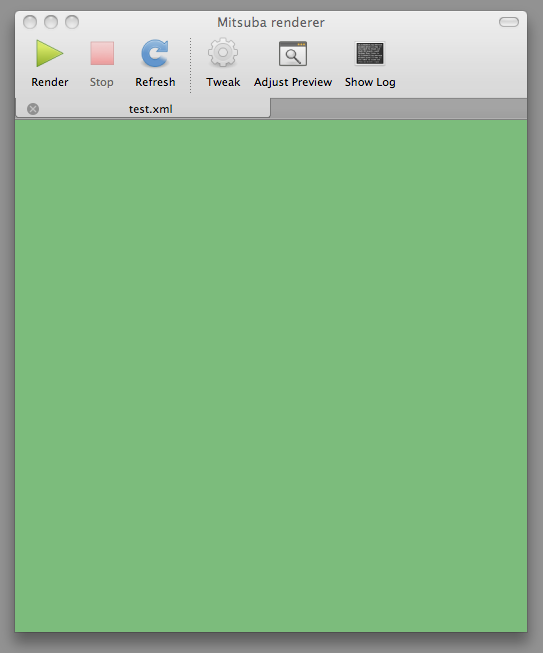
\includegraphics{images/integrator_green.png}}
\end{center}
That is admittedly not very exciting --- so let's do some actual computation.
\subsection{Visualizing depth}
Add an instance variable \code{Float m\_maxDist;} to the implementation. This
will store the maximum distance from the camera to any object, which is needed
to map distances into the $[0,1]$ range. Note the upper-case \code{Float} --- 
this means that either a single- or a double-precision variable is 
substituted based the compilation flags. This variable constitutes local
state, thus it must not be forgotten in the serialization- and unserialization routines:
append
\begin{cpp}
	m_maxDist = stream->readFloat();
\end{cpp}
and
\begin{cpp}
	stream->writeFloat(m_maxDist);
\end{cpp}
to the unserialization constructor and the \code{serialize} method, respectively.

We'll conservatively bound the maximum distance by measuring the
distance to all corners of the bounding box, which encloses the scene.
To avoid having to do this every time \code{Li()} is called,
we can override the \code{preprocess} function:
\begin{cpp}
	/// Preprocess function -- called on the initiating machine
	bool preprocess(const Scene *scene, RenderQueue *queue, 
			const RenderJob *job, int sceneResID, int cameraResID, 
			int samplerResID) {
		SampleIntegrator::preprocess(scene, queue, job, sceneResID, 
			cameraResID, samplerResID);

		const AABB &sceneAABB = scene->getAABB();
		Point cameraPosition = scene->getCamera()->getPosition();
		m_maxDist = - std::numeric_limits<Float>::infinity();

		for (int i=0; i<8; ++i)
			m_maxDist = std::max(m_maxDist, 
				(cameraPosition - sceneAABB.getCorner(i)).length());

		return true;
	}
\end{cpp}
The bottom of this function should be relatively self-explanatory. The
numerous arguments at the top are related to the parallelization layer, which will be
considered in more detail in the next section. Briefly, the render queue
provides synchronization facilities for render jobs (e.g. one can wait
for a certain job to terminate). And the integer parameters are
global resource identifiers. When a network render job runs, many associated
pieces of information (the scene, the camera, etc.) are wrapped into global resource chunks
shared amongst all nodes, and these can be referenced using such identifiers.

One important aspect of the \code{preprocess} function is that it is executed 
on the initiating node and before any of the parallel rendering begins. 
This can be used to compute certain things only once. Any
information updated here (such as \code{m\_maxDist}) will be forwarded to the
other nodes before the rendering begins.

Now, replace the body of the \code{Li} method with 
\begin{cpp}
	if (rRec.rayIntersect(r)) {
		Float distance = rRec.its.t;
		return Spectrum(1.0f - distance/m_maxDist) * m_color;
	}
	return Spectrum(0.0f);
\end{cpp}
and the distance renderer is done!
\begin{center}
\scalebox{.3}{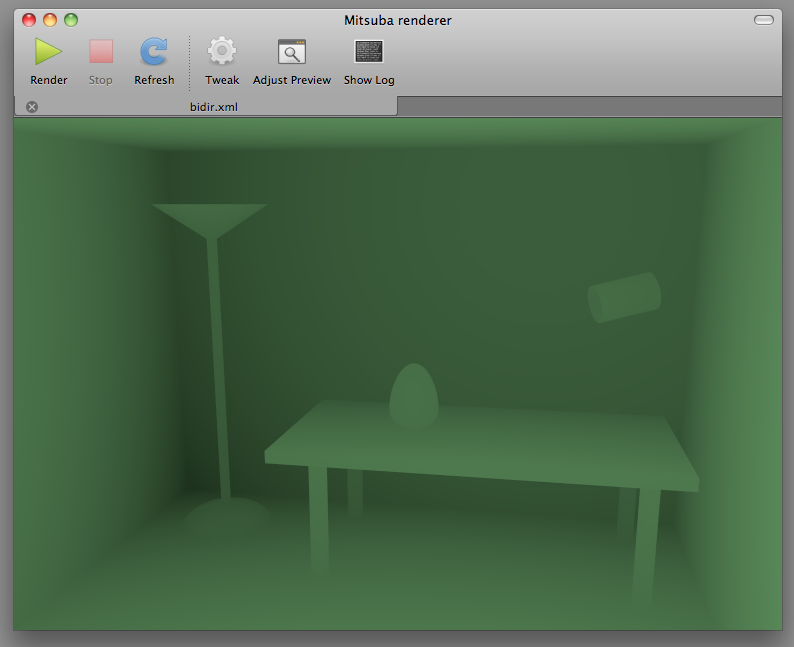
\includegraphics{images/integrator_depth.png}}
\end{center}
There are a few more noteworthy details: first of all, the ``usual'' way
to intersect a ray against the scene actually works like this:
\begin{cpp}
	Intersection its;
	Ray ray = ...;
	if (scene->rayIntersect(ray, its)) {
		/* Do something with the intersection stored in 'its' */
	}
\end{cpp}
As you can see, we did something slightly different in the distance 
renderer fragment above (we called \code{RadianceQueryRecord::rayIntersect()}
on the supplied parameter \code{rRec}), and the reason for this is \emph{nesting}.
\subsection{Nesting}
The idea of of nesting is that sampling-based rendering techniques can be
embedded within each other for added flexibility: for instance, one 
might concoct a  1-bounce indirect rendering technique complete with 
irradiance caching and adaptive integration simply by writing the following 
into a scene XML file:
\begin{xml}
<!-- Adaptively integrate using the nested technique -->
<integrator type="errctrl"> 
	<!-- Irradiance caching + final gathering with the nested technique -->
	<integrator type="irrcache"> 
		<!-- Simple direct illumination technique -->
		<integrator type="direct"> 
	</integrator>
</integrator>
\end{xml}
To support this kind of complex interaction, some information needs to be passed between the 
integrators, and the \code{RadianceQueryRecord} parameter of the function
\code{SampleIntegrator::Li} is used for this.

This brings us back to the odd way of computing an intersection a moment ago: 
the reason why we didn't just do this by calling  
\code{scene->rayIntersect()} is that our technique might actually be nested
within a parent technique, which has already computed this intersection.
To avoid wasting resources, the function \code{rRec.rayIntersect} first 
determines whether an intersection record has already been provided. 
If yes, it does nothing. Otherwise, it takes care of computing one. 

The radiance query record also lists the particular \emph{types} of radiance requested
by the parent integrator -- your implementation should respect these as much
as possible. Your overall code might for example be structured like this:

\begin{cpp}
   Spectrum Li(const RayDifferential &r, RadianceQueryRecord &rRec) const {
	  Spectrum result;
      if (rRec.type & RadianceQueryRecord::EEmittedRadiance) {
         // Emitted surface radiance contribution was requested
		 result += ...;
	  }
      if (rRec.type & RadianceQueryRecord::EDirectRadiance) {
         // Direct illumination contribution was requested
		 result += ...;
	  }
	  ...
	  return result;
   }
\end{cpp}

\section{Parallelization layer}
Mitsuba is built on top of a flexible parallelization layer, which spreads out
various types of computation over local and remote cores.
The guiding principle is that if an operation can potentially take longer than a
few seconds, it ought to use all the cores it can get.

Here, we will go through a basic example, which will hopefully provide sufficient intuition
to realize more complex tasks. 
To obtain good (i.e. close to linear) speedups, the parallelization layer depends on
several key assumptions of the task to be parallelized:
\begin{itemize}
\item The task can easily be split up into a discrete number of \emph{work units}, which requires a negligible amount of computation.
\item Each work unit is small in footprint so that it can easily be transferred over the network or shared memory. 
\item A work unit constitutes a significant amount of computation, which by far outweighs the cost of transmitting it to another node.
\item The \emph{work result} obtained by processing a work unit is again small in footprint, so that it can easily be transferred back.
\item Merging all work results to a solution of the whole problem requires a negligible amount of additional computation.
\end{itemize}
This essentially corresponds to a parallel version of \emph{Map} (one part of \emph{Map\&Reduce}) and is 
ideally suited for most rendering workloads. 

The example we consider here computes a \code{ROT13} ``encryption'' of a string, which 
most certainly violates the ``significant amount of computation'' assumption.
It was chosen due to the inherent parallelism and simplicity of this task.
While of course over-engineered to the extreme, the example hopefully 
communicates how this framework might be used in more complex scenarios.

We will implement this program as a plugin for the utility launcher \code{mtsutil}, which
frees us from having to write lots of code to set up the framework, prepare the
scheduler, etc.

We start by creating the utility skeleton file \code{src/utils/rot13.cpp}:
\begin{cpp}
#include <mitsuba/render/util.h>

MTS_NAMESPACE_BEGIN

class ROT13Encoder : public Utility {
public:
	ROT13Encoder(UtilityServices *us) : Utility(us) { }

	int run(int argc, char **argv) {
		cout << "Hello world!" << endl;
		return 0;
	}

	MTS_DECLARE_CLASS()
};

MTS_IMPLEMENT_CLASS(ROT13Encoder, false, Utility)
MTS_EXPORT_UTILITY(ROT13Encoder, "Perform a ROT13 encryption of a string")
MTS_NAMESPACE_END
\end{cpp}
The file must also be added to the build system: insert the line
\begin{shell}
plugins += $\texttt{env}$.SharedLibrary('plugins/rot13', ['src/utils/rot13.cpp'])
\end{shell}
into the SConscript (near the comment ``\code{Build the plugins -- utilities}''). After compiling
using \code{scons}, the \code{mtsutil} binary should automatically pick up your new utility plugin:
\begin{shell}
$\texttt{\$}$ mtsutil
..
The following utilities are available:

	addimages             Generate linear combinations of EXR images
	rot13                 Perform a ROT13 encryption of a string
\end{shell}
It can be executed as follows:
\begin{shell}
$\texttt{\$}$ mtsutil rot13
2010-08-16 18:38:27 INFO  main [src/mitsuba/mtsutil.cpp:276] Mitsuba version 0.1.1, Copyright (c) 2010 Wenzel Jakob
2010-08-16 18:38:27 INFO  main [src/mitsuba/mtsutil.cpp:350] Loading utility "rot13" ..
Hello world!
\end{shell}

Our approach for implementing distributed ROT13 will be to treat each character as an 
indpendent work unit. Since the ordering is lost when sending out work units, we must
also include the position of the character in both the work units and the work results.

All of the relevant interfaces are contained in \code{include/mitsuba/core/sched.h}.
For reference, here are the interfaces of \code{WorkUnit} and \code{WorkResult}:
\newpage
\begin{cpp}
/**
 * Abstract work unit. Represents a small amount of information
 * that encodes part of a larger processing task. 
 */
class MTS_EXPORT_CORE WorkUnit : public Object {
public:
	/// Copy the content of another work unit of the same type
	virtual void set(const WorkUnit *workUnit) = 0;

	/// Fill the work unit with content acquired from a binary data stream
	virtual void load(Stream *stream) = 0;

	/// Serialize a work unit to a binary data stream
	virtual void save(Stream *stream) const = 0;

	/// Return a string representation
	virtual std::string toString() const = 0;

	MTS_DECLARE_CLASS()
protected:
	/// Virtual destructor
	virtual ~WorkUnit() { }
};
/**
 * Abstract work result. Represents the information that encodes 
 * the result of a processed <tt>WorkUnit</tt> instance.
 */
class MTS_EXPORT_CORE WorkResult : public Object {
public:
	/// Fill the work result with content acquired from a binary data stream
	virtual void load(Stream *stream) = 0;

	/// Serialize a work result to a binary data stream
	virtual void save(Stream *stream) const = 0;

	/// Return a string representation
	virtual std::string toString() const = 0;

	MTS_DECLARE_CLASS()
protected:
	/// Virtual destructor
	virtual ~WorkResult() { }
};
\end{cpp}
\newpage
In our case, the \code{WorkUnit} implementation then looks like this:
\begin{cpp}
class ROT13WorkUnit : public WorkUnit {
public:
	void set(const WorkUnit *workUnit) {
		const ROT13WorkUnit *wu = 
			static_cast<const ROT13WorkUnit *>(workUnit);
		m_char = wu->m_char;
		m_pos = wu->m_pos;
	}

	void load(Stream *stream) {
		m_char = stream->readChar();
		m_pos = stream->readInt();
	}
	
	void save(Stream *stream) const {
		stream->writeChar(m_char);
		stream->writeInt(m_pos); 
	}

	std::string toString() const {
		std::ostringstream oss;
		oss << "ROT13WorkUnit[" << endl
			<< "  char = '" << m_char << "'," << endl
			<< "  pos = " << m_pos << endl
			<< "]";
		return oss.str();
	}

	inline char getChar() const { return m_char; }
	inline void setChar(char value) { m_char = value; }
	inline int getPos() const { return m_pos; }
	inline void setPos(int value) { m_pos = value; }

	MTS_DECLARE_CLASS()
private:
	char m_char;
	int m_pos;
};

MTS_IMPLEMENT_CLASS(ROT13WorkUnit, false, WorkUnit)
\end{cpp}
The \code{ROT13WorkResult} implementation is not reproduced since it is almost identical 
(except that it doesn't need the \code{set} method).
The similarity is not true in general: for most algorithms, the work unit and result 
will look completely different.

Next, we need a class, which does the actual work of turning a work unit into a work result
(a subclass of \code{WorkProcessor}). Again, we need to implement a range of support
methods to enable the various ways in which work processor instances will be submitted to 
remote worker nodes and replicated amongst local threads.
\begin{cpp}
class ROT13WorkProcessor : public WorkProcessor {
public:
	/// Construct a new work processor
	ROT13WorkProcessor() : WorkProcessor() { }

	/// Unserialize from a binary data stream (nothing to do in our case)
	ROT13WorkProcessor(Stream *stream, InstanceManager *manager)
		: WorkProcessor(stream, manager) { }

	/// Serialize to a binary data stream (nothing to do in our case)
	void serialize(Stream *stream, InstanceManager *manager) const {
	}

	ref<WorkUnit> createWorkUnit() const {
		return new ROT13WorkUnit();
	}

	ref<WorkResult> createWorkResult() const { 
		return new ROT13WorkResult();
	}

	ref<WorkProcessor> clone() const {
		return new ROT13WorkProcessor(); // No state to clone in our case
	}

	/// No internal state, thus no preparation is necessary
	void prepare() { }

	/// Do the actual computation
	void process(const WorkUnit *workUnit, WorkResult *workResult, 
				 const bool &stop) {
		const ROT13WorkUnit *wu 
			= static_cast<const ROT13WorkUnit *>(workUnit);
		ROT13WorkResult *wr = static_cast<ROT13WorkResult *>(workResult);
		wr->setPos(wu->getPos());
		wr->setChar((std::toupper(wu->getChar()) - 'A' + 13) % 26 + 'A');
	}
	MTS_DECLARE_CLASS()
};
MTS_IMPLEMENT_CLASS_S(ROT13WorkProcessor, false, WorkProcessor)
\end{cpp}
Since our work processor has no state, most of the implementations
are rather trivial. Note the \code{stop} field in the \code{process}
method. This field is used to abort running jobs at the users requests, hence
it is a good idea to periodically check its value during lengthy computations.

Finally, we need a called \emph{parallel process}
instance, which is responsible for creating work units and stitching
work results back into a solution of the whole problem. The \code{ROT13}
implementation might look as follows:
\begin{cpp}
class ROT13Process : public ParallelProcess {
public:
	ROT13Process(const std::string &input) : m_input(input), m_pos(0) {
		m_output.resize(m_input.length());
	}

	ref<WorkProcessor> createWorkProcessor() const {
		return new ROT13WorkProcessor();
	}

	std::vector<std::string> getRequiredPlugins() {
		std::vector<std::string> result;
		result.push_back("rot13");
		return result;
	}

	EStatus generateWork(WorkUnit *unit, int worker /* unused */) {
		if (m_pos >= (int) m_input.length())
			return EFailure;
		ROT13WorkUnit *wu = static_cast<ROT13WorkUnit *>(unit);

		wu->setPos(m_pos);
		wu->setChar(m_input[m_pos++]);

		return ESuccess;
	}

	void processResult(const WorkResult *result, bool cancelled) {
		if (cancelled) // indicates a work unit, which was 
			return;    // cancelled partly through its execution
		const ROT13WorkResult *wr = 
			static_cast<const ROT13WorkResult *>(result);
		m_output[wr->getPos()] = wr->getChar();
	}

	inline const std::string &getOutput() {
		return m_output;
	}

	MTS_DECLARE_CLASS()
public:
	std::string m_input;
	std::string m_output;
	int m_pos;
};
MTS_IMPLEMENT_CLASS(ROT13Process, false, ParallelProcess)
\end{cpp}
The \code{generateWork} method produces work units until we have moved past
the end of the string, after which it returns the status code \code{EFailure}.
Note the method \code{getRequiredPlugins()}: this is necessary to use 
the utility across
machines. When communicating with another node, it ensures that the remote side
loads the \code{ROT13*} classes at the right moment.

To actually use the \code{ROT13} encoder, we must first launch the newly created parallel process
from the main utility function (the `Hello World' code we wrote earlier). We can adapt it as follows:
\begin{cpp}
	int run(int argc, char **argv) {
		if (argc < 2) {
			cout << "Syntax: mtsutil rot13 <text>" << endl;
			return -1;
		}

		ref<ROT13Process> proc = new ROT13Process(argv[1]);
		ref<Scheduler> sched = Scheduler::getInstance();

		/* Submit the encryption job to the scheduler */
		sched->schedule(proc);

		/* Wait for its completion */
		sched->wait(proc);

		cout << "Result: " << proc->getOutput() << endl;

		return 0;
	}
\end{cpp}
After compiling everything using \code{scons}, an exemplary usage
would be to encode a string (e.g. \code{SECUREBYDESIGN}), while 
forwarding all computation to a network machine. (\code{-p0} disables
all local worker threads). Adding a verbose flag (\code{-v}) shows 
some additional scheduling information:
\begin{shell}
$\texttt{\$}$ mtsutil -vc feynman -p0 rot13 SECUREBYDESIGN
2010-08-17 01:35:46 INFO  main [src/mitsuba/mtsutil.cpp:201] Mitsuba version 0.1.1, Copyright (c) 2010 Wenzel Jakob
2010-08-17 01:35:46 INFO  main [SocketStream] Connecting to "feynman:7554"
2010-08-17 01:35:46 DEBUG main [Thread] Spawning thread "net0_r"
2010-08-17 01:35:46 DEBUG main [RemoteWorker] Connection to "feynman" established (2 cores).
2010-08-17 01:35:46 DEBUG main [Scheduler] Starting ..
2010-08-17 01:35:46 DEBUG main [Thread] Spawning thread "net0"
2010-08-17 01:35:46 INFO  main [src/mitsuba/mtsutil.cpp:275] Loading utility "rot13" ..
2010-08-17 01:35:46 DEBUG main [Scheduler] Scheduling process 0: ROT13Process[unknown]..
2010-08-17 01:35:46 DEBUG main [Scheduler] Waiting $\texttt{for}$ process 0
2010-08-17 01:35:46 DEBUG net0 [Scheduler] Process 0 has finished generating work
2010-08-17 01:35:46 DEBUG net0_r[Scheduler] Process 0 is $\texttt{complete}$.
Result: FRPHEROLQRFVTA
2010-08-17 01:35:46 DEBUG main [Scheduler] Pausing ..
2010-08-17 01:35:46 DEBUG net0 [Thread] Thread "net0" has finished
2010-08-17 01:35:46 DEBUG main [Scheduler] Stopping ..
2010-08-17 01:35:46 DEBUG main [RemoteWorker] Shutting down
2010-08-17 01:35:46 DEBUG net0_r[Thread] Thread "net0_r" has finished
\end{shell}
\subsection{Global Resources}
TBD.

\section{Python integration}
\label{sec:python}
A recent feature of Mitsuba is a Python interface to the renderer API.
While the interface is still limited at this point, it can already be
used for many useful purposes. To access the API, start your Python
interpreter and enter
\begin{python}
import mitsuba
\end{python}
\paragraph{Mac OS:}
For this to work on MacOS X, you will first have to run the ``\emph{Apple
Menu}$\to$\emph{Command-line access}'' menu item from within Mitsuba.
In the unlikely case that you run into shared library loading issues (this is
taken care of by default), you may have to set the \code{LD\_LIBRARY\_PATH}
environment variable before starting Python so that it points to where the
Mitsuba libraries are installed (e.g. the \code{Mitsuba.app/Contents/Frameworks}
directory).

When Python crashes directly after the \code{import mitsuba} statement,
make sure that Mitsuba is linked against the right Python distribution
(i.e. matching the \code{python} binary you are using). For e.g. Python
2.7, can be done by adjusting the \code{PYTHON27INCLUDE} and
\code{PYTHON27LIBDIR} variables in \code{config.py}. For other versions,
adjust the numbers accordingly.

\paragraph{Windows and Linux:}
On Windows and \emph{non-packaged} Linux builds, you may have to explicitly
specify the required extension search path before issuing the \code{import} command, e.g.:
\begin{python}
import os, sys

# Specify the extension search path on Linux/Windows (may vary depending on your
# setup. If you compiled from  source, 'path-to-mitsuba-directory' should be the
# 'dist' subdirectory)

# NOTE: On Windows, specify these paths using FORWARD slashes (i.e. '/' instead of
# '\' to avoid pitfalls with string escaping)

# Configure the search path for the Python extension module
sys.path.append('path-to-mitsuba-directory/python/<python version, e.g. 2.7>')

# Ensure that Python will be able to find the Mitsuba core libraries
os.environ['PATH'] = 'path-to-mitsuba-directory' + os.pathsep + os.environ['PATH']

import mitsuba
\end{python}
In rare cases when running on Linux, it may also be necessary to set the
\code{LD\_LIBRARY\_PATH} environment variable before starting Python so that it
points to where the Mitsuba core libraries are installed.

For an overview of the currently exposed API subset, please refer
to the following page: \url{http://www.mitsuba-renderer.org/api/group__libpython.html}.

\subsubsection*{Accessing signatures in an interactive Python shell}
The plugin exports comprehensive Python-style docstrings, hence
the following is an alternative and convenient way of getting information on
classes, function, or entire namespaces when running an interactive Python shell.
\begin{shell}
>>> help(mitsuba.core.Bitmap) # (can be applied to namespaces, classes, functions, etc.)

 class Bitmap(Object)
  |  Method resolution order:
  |      Bitmap
  |      Object
  |      Boost.Python.instance
  |      __builtin__.object
  |
  |  Methods defined here:
  |  __init__(...)
  |      __init__( (object)arg1, (EPixelFormat)arg2, (EComponentFormat)arg3, (Vector2i)arg4) -> None :
  |          C++ signature :
  |              void __init__(_object*,mitsuba::Bitmap::EPixelFormat,mitsuba::Bitmap::EComponentFormat,mitsuba::TVector2<int>)
  |
  |      __init__( (object)arg1, (EFileFormat)arg2, (Stream)arg3) -> None :
  |          C++ signature :
  |              void __init__(_object*,mitsuba::Bitmap::EFileFormat,mitsuba::Stream*)
  |
  |  clear(...)
  |      clear( (Bitmap)arg1) -> None :
  |          C++ signature :
  |              void clear(mitsuba::Bitmap {lvalue})
...
\end{shell}
The docstrings list the currently exported functionality, as well as C++ and Python signatures, but they
don't document what these functions actually do. The web API documentation is
the preferred source of this information.

\subsection{Basics}
Generally, the Python API tries to mimic the C++ API as closely as possible.
Where applicable, the Python classes and methods replicate overloaded operators,
overridable virtual function calls, and default arguments. Under rare circumstances,
some features are inherently non-portable due to fundamental differences between the
two programming languages. In this case, the API documentation will contain further
information.

Mitsuba's linear algebra-related classes are usable with essentially the
same syntax as their C++ versions --- for example, the following snippet
creates and rotates a unit vector.
\begin{python}
import mitsuba
from mitsuba.core import *

# Create a normalized direction vector
myVector = normalize(Vector(1.0, 2.0, 3.0))

# 90 deg. rotation around the Y axis
trafo = Transform.rotate(Vector(0, 1, 0), 90)

# Apply the rotation and display the result
print(trafo * myVector)
\end{python}

\subsection{Recipes}
The following section contains a series of ``recipes'' on how to do
certain things with the help of the Python bindings.

\subsubsection{Loading a scene}
The following script demonstrates how to use the
\code{FileResolver} and \code{SceneHandler} classes to
load a Mitsuba scene from an XML file:
\begin{python}
import mitsuba

from mitsuba.core import *
from mitsuba.render import SceneHandler

# Get a reference to the thread's file resolver
fileResolver = Thread.getThread().getFileResolver()

# Register any searchs path needed to load scene resources (optional)
fileResolver.appendPath('<path to scene directory>')

# Optional: supply parameters that can be accessed
# by the scene (e.g. as $\text{\color{lstcomment}\itshape\texttt{\$}}$myParameter)
paramMap = StringMap()
paramMap['myParameter'] = 'value'

# Load the scene from an XML file
scene = SceneHandler.loadScene(fileResolver.resolve("scene.xml"), paramMap)

# Display a textual summary of the scene's contents
print(scene)
\end{python}

\subsubsection{Rendering a loaded scene}
Once a scene has been loaded, it can be rendered as follows:
\begin{python}
from mitsuba.core import *
from mitsuba.render import RenderQueue, RenderJob
import multiprocessing

scheduler = Scheduler.getInstance()

# Start up the scheduling system with one worker per local core
for i in range(0, multiprocessing.cpu_count()):
	scheduler.registerWorker(LocalWorker(i, 'wrk%i' % i))
scheduler.start()

# Create a queue for tracking render jobs
queue = RenderQueue()

scene.setDestinationFile('renderedResult')

# Create a render job and insert it into the queue
job = RenderJob('myRenderJob', scene, queue)
job.start()

# Wait for all jobs to finish and release resources
queue.waitLeft(0)
queue.join()

# Print some statistics about the rendering process
print(Statistics.getInstance().getStats())
\end{python}

\subsubsection{Rendering over the network}
To render over the network, you must first set up one or
more machines that run the \code{mtssrv} server (see \secref{mtssrv}).
A network node can then be registered with the scheduler as follows:
\begin{python}
# Connect to a socket on a named host or IP address
# 7554 is the default port of 'mtssrv'
stream = SocketStream('128.84.103.222', 7554)

# Create a remote worker instance that communicates over the stream
remoteWorker = RemoteWorker('netWorker', stream)

scheduler = Scheduler.getInstance()
# Register the remote worker (and any other potential workers)
scheduler.registerWorker(remoteWorker)
scheduler.start()
\end{python}

\subsubsection{Constructing custom scenes from Python}
Dynamically constructing Mitsuba scenes entails loading a series of external
plugins, instantiating them with custom parameters, and finally assembling
them into an object graph.
For instance, the following snippet shows how to create a basic
perspective sensor with a film that writes PNG images:
\begin{python}
from mitsuba.core import *
pmgr = PluginManager.getInstance()

# Encodes parameters on how to instantiate the 'perspective' plugin
sensorProps = Properties('perspective')
sensorProps['toWorld'] = Transform.lookAt(
	Point(0, 0, -10),  # Camera origin
	Point(0, 0, 0),    # Camera target
	Vector(0, 1, 0)    # 'up' vector
)
sensorProps['fov'] = 45.0

# Encodes parameters on how to instantiate the 'ldrfilm' plugin
filmProps = Properties('ldrfilm')
filmProps['width'] = 1920
filmProps['height'] = 1080

# Load and instantiate the plugins
sensor = pmgr.createObject(sensorProps)
film = pmgr.createObject(filmProps)

# First configure the film and then add it to the sensor
film.configure()
sensor.addChild('film', film)

# Now, the sensor can be configured
sensor.configure()
\end{python}
The above code fragment uses the plugin manager to construct a
\code{Sensor} instance from an external plugin named
\texttt{perspective.so/dll/dylib} and adds a child object
named \texttt{film}, which is a \texttt{Film} instance loaded from the
plugin \texttt{ldrfilm.so/dll/dylib}.
Each time after instantiating a plugin, all child objects are added, and
finally the  plugin's \code{configure()} method must be called.

Creating scenes in this manner ends up being rather laborious.
Since Python comes with a powerful dynamically-typed dictionary
primitive, Mitsuba additionally provides a more ``pythonic''
alternative that makes use of this facility:
\begin{python}
from mitsuba.core import *

pmgr = PluginManager.getInstance()
sensor = pmgr.create({
	'type' : 'perspective',
	'toWorld' : Transform.lookAt(
		Point(0, 0, -10),
		Point(0, 0, 0),
		Vector(0, 1, 0)
	),
	'film' : {
		'type' : 'ldrfilm',
		'width' : 1920,
		'height' : 1080
	}
})
\end{python}
This code does exactly the same as the previous snippet.
By the time \code{PluginManager.create} returns, the object
hierarchy has already been assembled, and the
\code{configure()} method of every object
has been called.

Finally, here is an full example that creates a basic scene
which can be rendered. It describes a sphere lit by a point
light, rendered using the direct illumination integrator.
\begin{python}
from mitsuba.core import *
from mitsuba.render import Scene

scene = Scene()

# Create a sensor, film & sample generator
scene.addChild(pmgr.create({
	'type' : 'perspective',
	'toWorld' : Transform.lookAt(
		Point(0, 0, -10),
		Point(0, 0, 0),
		Vector(0, 1, 0)
	),
	'film' : {
		'type' : 'ldrfilm',
		'width' : 1920,
		'height' : 1080
	},
	'sampler' : {
		'type' : 'ldsampler',
		'sampleCount' : 2
	}
}))

# Set the integrator
scene.addChild(pmgr.create({
	'type' : 'direct'
}))

# Add a light source
scene.addChild(pmgr.create({
	'type' : 'point',
	'position' : Point(5, 0, -10),
	'intensity' : Spectrum(100)
}))

# Add a shape
scene.addChild(pmgr.create({
	'type' : 'sphere',
	'center' : Point(0, 0, 0),
	'radius' : 1.0,
	'bsdf' : {
		'type' : 'diffuse',
		'reflectance' : Spectrum(0.4)
	}
}))

scene.configure()
\end{python}

\subsubsection{Taking control of the logging system}
Many operations in Mitsuba will print one or more log messages
during their execution. By default, they will be printed to the console,
which may be undesirable. Similar to the C++ side, it is possible to define
custom \code{Formatter} and \code{Appender} classes to interpret and direct
the flow of these messages. This is also useful to keep track of the progress
of rendering jobs.

Roughly, a \code{Formatter} turns detailed
information about a logging event into a human-readable string, and a
\code{Appender} routes it to some destination (e.g. by appending it to
a file or a log viewer in a graphical user interface). Here is an example
of how to activate such extensions:
\begin{python}
import mitsuba
from mitsuba.core import *

class MyFormatter(Formatter):
	def format(self, logLevel, sourceClass, sourceThread, message, filename, line):
		return '%s (log level: %s, thread: %s, class %s, file %s, line %i)' % \
				(message, str(logLevel), sourceThread.getName(), sourceClass,
				 filename, line)

class MyAppender(Appender):
	def append(self, logLevel, message):
		print(message)

	def logProgress(self, progress, name, formatted, eta):
		print('Progress message: ' + formatted)

# Get the logger associated with the current thread
logger = Thread.getThread().getLogger()
logger.setFormatter(MyFormatter())
logger.clearAppenders()
logger.addAppender(MyAppender())
logger.setLogLevel(EDebug)

Log(EInfo, 'Test message')
\end{python}
\subsubsection{Rendering a turntable animation with motion blur}
Rendering a turntable animation is a fairly common task that is
conveniently accomplished via the Python interface. In a turntable
video, the camera rotates around a completely static object or scene.
The following snippet does this for the material test ball scene downloadable
on the main website, complete with motion blur. It assumes that the
scene and scheduler have been set up approriately using one of the previous
snippets.
\begin{python}
sensor = scene.getSensor()
sensor.setShutterOpen(0)
sensor.setShutterOpenTime(1)

stepSize = 5
for i in range(0,360 / stepSize):
    rotationCur  = Transform.rotate(Vector(0, 0, 1), i*stepSize);
    rotationNext = Transform.rotate(Vector(0, 0, 1), (i+1)*stepSize);

    trafoCur  = Transform.lookAt(rotationCur  * Point(0,-6,4),
        Point(0, 0, .5), rotationCur  * Vector(0, 1, 0))
    trafoNext = Transform.lookAt(rotationNext * Point(0,-6,4),
        Point(0, 0, .5), rotationNext * Vector(0, 1, 0))

    atrafo = AnimatedTransform()
    atrafo.appendTransform(0, trafoCur)
    atrafo.appendTransform(1, trafoNext)
    atrafo.sortAndSimplify()
    sensor.setWorldTransform(atrafo)

    scene.setDestinationFile('frame_%03i.png' % i)
    job = RenderJob('job_%i' % i, scene, queue)
    job.start()

    queue.waitLeft(0)
    queue.join()
\end{python}
A useful property of this approach is that scene loading and initialization
must only take place once. Performance-wise, this compares favourably with
running many separate rendering jobs, e.g. using the \code{mitsuba}
command-line executable.

\subsubsection{Creating triangle-based shapes}
It is possible to create new triangle-based shapes directly in Python, though
doing so is discouraged: because Python is an interpreted programming language,
the construction of large meshes will run very slowly. The builtin shapes
and shape loaders are to be preferred when this is an option. That said, the
following snippet shows how to create \code{TriMesh} objects from within Python:
\begin{python}
# Create a new mesh with 1 triangle, 3 vertices,
# and allocate buffers for normals and texture coordinates
mesh = TriMesh('Name of this mesh', 1, 3, True, True)

v = mesh.getVertexPositions()
v[0] = Point3(0, 0, 0)
v[1] = Point3(1, 0, 0)
v[2] = Point3(0, 1, 0)

n = mesh.getVertexNormals()
n[0] = Normal(0, 0, 1)
n[1] = Normal(0, 0, 1)
n[2] = Normal(0, 0, 1)

t = mesh.getTriangles() # Indexed triangle list: tri 1 references vertices 0,1,2
t[0] = 0
t[1] = 1
t[2] = 2

uv = mesh.getTexcoords()
uv[0] = Point2(0, 0)
uv[1] = Point2(1, 0)
uv[2] = Point2(0, 1)

mesh.configure()

# Add to a scene (assumes 'scene' is available)
sensor.addChild(mesh)
\end{python}


\subsubsection{Calling Mitsuba functions from a multithread Python program}
By default, Mitsuba assumes that threads accessing Mitsuba-internal
data structures were created by (or at least registered with) Mitsuba. This is the
case for the main thread and subclasses of \code{mitsuba.core.Thread}. When a
Mitsuba function is called from an event dispatch thread of a multithreaded
Python application that is not known to Mitsuba, an exception or crash will result.

To avoid this, get a reference to the main thread right after loading the Mitsuba plugin
and save some related state (the attached \code{FileResolver} and \code{Logger} instances).
\begin{python}
mainThread = Thread.getThead()
saved_fresolver = mainThread.getFileResolver()
saved_logger = mainThread.getLogger()
\end{python}

Later when accessed from an unregister thread, execute the following:
\begin{python}
# This rendering thread was not created by Mitsuba -- register it
newThread = Thread.registerUnmanagedThread('render')
newThread.setFileResolver(saved_fresolver)
newThread.setLogger(saved_logger)
\end{python}
It is fine to execute this several times (\code{registerUnmanagedThread} just returns
a reference to the associated \code{Thread} instance if it was already registered).

\subsubsection{PyQt/PySide interaction with Mitsuba (simple version)}
The following listing contains a complete program that
renders a sphere and efficiently displays it in a PyQt window
(to make this work in PySide, change all occurrences of \code{PyQt4} to \code{PySide} in the
import declarations and rename the function call to \code{getNativeBuffer()} to \code{toByteArray()},
which is a tiny bit less efficient).
\begin{python}
import mitsuba, multiprocessing, sys

from mitsuba.core import Scheduler, PluginManager, \
    LocalWorker, Properties, Bitmap, Point2i, FileStream

from mitsuba.render import RenderQueue, RenderJob, Scene

from PyQt4.QtCore import QPoint
from PyQt4.QtGui import QApplication, QMainWindow, QPainter, QImage

class MitsubaView(QMainWindow):
    def __init__(self):
        super(MitsubaView, self).__init__()
        self.setWindowTitle('Mitsuba/Qt demo')
        self.initializeMitsuba()
        self.image = self.render(self.createScene())
        self.resize(self.image.width(), self.image.height())

    def initializeMitsuba(self):
        # Start up the scheduling system with one worker per local core
        self.scheduler = Scheduler.getInstance()
        for i in range(0, multiprocessing.cpu_count()):
            self.scheduler.registerWorker(LocalWorker(i, 'wrk%i' % i))
        self.scheduler.start()
        # Create a queue for tracking render jobs
        self.queue = RenderQueue()
        # Get a reference to the plugin manager
        self.pmgr = PluginManager.getInstance()

    def shutdownMitsuba(self):
        self.queue.join()
        self.scheduler.stop()

    def createScene(self):
        # Create a simple scene containing a sphere
        sphere = self.pmgr.createObject(Properties("sphere"))
        sphere.configure()
        scene = Scene()
        scene.addChild(sphere)
        scene.configure()
        # Don't automatically write an output bitmap file when the
        # rendering process finishes (want to control this from Python)
        scene.setDestinationFile('')
        return scene

    def render(self, scene):
        # Create a render job and insert it into the queue
        job = RenderJob('myRenderJob', scene, self.queue)
        job.start()
        # Wait for the job to finish
        self.queue.waitLeft(0)
        # Develop the camera's film into an 8 bit sRGB bitmap
        film = scene.getFilm()
        size = film.getSize()
        bitmap = Bitmap(Bitmap.ERGB, Bitmap.EUInt8, size)
        film.develop(Point2i(0, 0), size, Point2i(0, 0), bitmap)
        # Write to a PNG bitmap file
        outFile = FileStream("rendering.png", FileStream.ETruncReadWrite)
        bitmap.write(Bitmap.EPNG, outFile)
        outFile.close()
        # Also create a QImage (using a fast memory copy in C++)
        return QImage(bitmap.getNativeBuffer(),
            size.x, size.y, QImage.Format_RGB888)

    def paintEvent(self, event):
        painter = QPainter(self)
        painter.drawImage(QPoint(0, 0), self.image)
        del painter

def main():
    app = QApplication(sys.argv)
    view = MitsubaView()
    view.show()
    view.raise_()
    retval = app.exec_()
    view.shutdownMitsuba()
    sys.exit(retval)

if __name__ == '__main__':
    main()
\end{python}

\subsubsection{PyQt/PySide interaction with Mitsuba (fancy)}
The following snippet is a much fancier version of the previous PyQt/PySide example.
Instead of waiting for the rendering to finish and then displaying it, this example launches the
rendering in the background and uses Mitsuba's \code{RenderListener} interface to update the
view and show image blocks as they are being rendered.
As before, some changes will be necessary to get this to run on PySide.
\begin{center}
    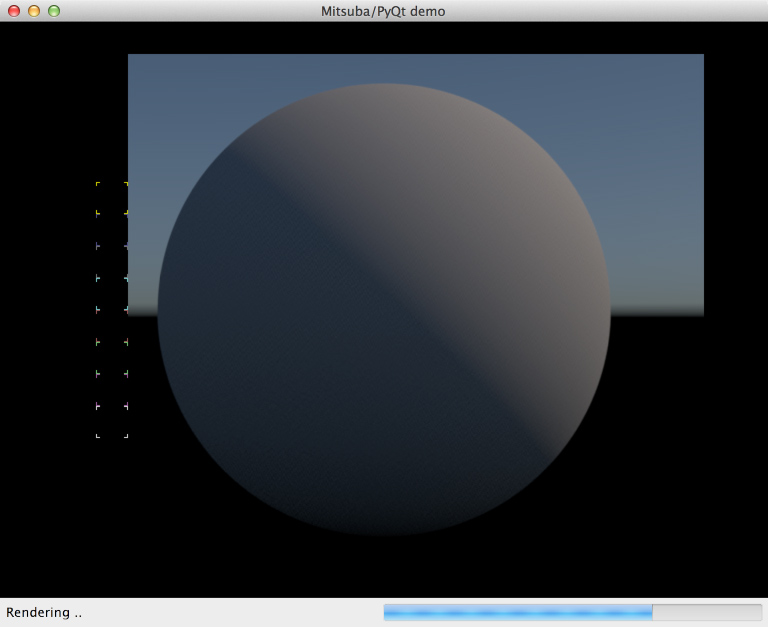
\includegraphics[width=10cm]{images/python_demo.jpg}
\end{center}
When using this snippet, please be wary of threading-related issues; the key thing to remember is that
in Qt, only the main thread is allowed to modify Qt widgets. On the other hand, rendering and logging-related
callbacks will be invoked from different Mitsuba-internal threads---this means that it's not possible to e.g.
directly update the status bar message from the callback \code{finishJobEvent}. To do this, we must use
use Qt's \code{QueuedConnection} to communicate this event to the main thread via signals and slots. See the
code that updates the status and progress bar for more detail.
\begin{python}
import mitsuba, multiprocessing, sys, time

from mitsuba.core import Scheduler, PluginManager, Thread, Vector, Point2i, \
    LocalWorker, Properties, Bitmap, Spectrum, Appender, EWarn, Transform, FileStream

from mitsuba.render import RenderQueue, RenderJob, Scene, RenderListener

from PyQt4.QtCore import Qt, QPoint, pyqtSignal
from PyQt4.QtGui import QApplication, QMainWindow, QPainter, QImage, QProgressBar

class MitsubaView(QMainWindow):
    viewUpdated = pyqtSignal()
    renderProgress = pyqtSignal(int)
    renderingCompleted = pyqtSignal(bool)

    def __init__(self):
        super(MitsubaView, self).__init__()
        self.setWindowTitle('Mitsuba/Qt demo')
        self.initializeMitsuba()
        self.qimage = self.render(self.createScene())
        status = self.statusBar()
        status.setContentsMargins(0,0,5,0)
        self.progress = QProgressBar(status)
        status.addPermanentWidget(self.progress)
        status.setSizeGripEnabled(False)
        self.setFixedSize(self.qimage.width(), self.qimage.height() +
            self.progress.height()*1.5)

        def handleRenderingCompleted(cancelled):
            status.showMessage("Rendering finished.")
            self.progress.setVisible(False)

            if not cancelled:
                outFile = FileStream("rendering.png", FileStream.ETruncReadWrite)
                self.bitmap.write(Bitmap.EPNG, outFile)
                outFile.close()

        self.viewUpdated.connect(self.repaint, Qt.QueuedConnection)
        self.renderProgress.connect(self.progress.setValue, Qt.QueuedConnection)
        self.renderingCompleted.connect(handleRenderingCompleted,
            Qt.QueuedConnection)
        status.showMessage("Rendering ..")

    def initializeMitsuba(self):
        # Start up the scheduling system with one worker per local core
        self.scheduler = Scheduler.getInstance()
        for i in range(0, multiprocessing.cpu_count()):
            self.scheduler.registerWorker(LocalWorker(i, 'wrk%i' % i))
        self.scheduler.start()
        # Create a queue for tracking render jobs
        self.queue = RenderQueue()
        # Get a reference to the plugin manager
        self.pmgr = PluginManager.getInstance()
        # Appender to process log and progress messages within Python
        class CustomAppender(Appender):
            def append(self2, logLevel, message):
                print(message)
            def logProgress(self2, progress, name, formatted, eta):
                self.renderProgress.emit(progress)

        logger = Thread.getThread().getLogger()
        logger.setLogLevel(EWarn)
        logger.clearAppenders()
        logger.addAppender(CustomAppender())

    def closeEvent(self, e):
        self.job.cancel()
        self.queue.join()
        self.scheduler.stop()

    def createScene(self):
        scene = self.pmgr.create({
            'type' : 'scene',
            'sphere' : {
                'type' : 'sphere',
            },
            'envmap' : {
                'type' : 'sunsky'
            },
            'sensor' : {
                'type' : 'perspective',
                'toWorld' : Transform.translate(Vector(0, 0, -5)),
                'sampler' : {
                    'type' : 'halton',
                    'sampleCount' : 64
                }
            }
        })
        return scene

    def render(self, scene):
        film = scene.getFilm()
        size = film.getSize()

        # Bitmap that will store pixels of the developed film
        self.bitmap = Bitmap(Bitmap.ERGB, Bitmap.EUInt8, size)
        self.bitmap.clear()

        # Listener to update bitmap subregions when blocks finish rendering
        class CustomListener(RenderListener):
            def __init__(self):
                super(CustomListener, self).__init__()
                self.time = 0
            def workBeginEvent(self2, job, wu, thr):
                self.bitmap.drawRect(wu.getOffset(), wu.getSize(), Spectrum(1.0))
                now = time.time()
                if now - self2.time > .25:
                    self.viewUpdated.emit()
                    self2.time = now
            def workEndEvent(self2, job, wr):
                film.develop(wr.getOffset(), wr.getSize(),
                    wr.getOffset(), self.bitmap)
                now = time.time()
                if now - self2.time > .25:
                    self.viewUpdated.emit()
                    self2.time = now
            def refreshEvent(self2, job):
                film.develop(Point2i(0), size, Point2i(0), self.bitmap)
                self.viewUpdated.emit()
            def finishJobEvent(self2, job, cancelled):
                self2.refreshEvent(job)
                self.renderingCompleted.emit(cancelled)

        # Create a render job and insert it into the queue
        self.job = RenderJob('rjob', scene, self.queue)
        self.queue.registerListener(CustomListener())
        self.job.start()

        # Return a QImage that directly points into the contents of self.bitmap
        return QImage(self.bitmap.getNativeBuffer(),
            size.x, size.y, QImage.Format_RGB888)

    def keyPressEvent(self, e):
        if e.key() == Qt.Key_Escape:
            self.close()

    def paintEvent(self, event):
        super(MitsubaView, self).paintEvent(event)
        painter = QPainter(self)
        painter.drawImage(QPoint(0, 0), self.qimage)
        del painter

def main():
    import signal
    # Stop the program upon Ctrl-C (SIGINT)
    signal.signal(signal.SIGINT, signal.SIG_DFL)

    app = QApplication(sys.argv)
    view = MitsubaView()
    view.show()
    view.raise_()
    retval = app.exec_()
    sys.exit(retval)

if __name__ == '__main__':
    main()
\end{python}


\section{Acknowledgments}
I am indebted to my advisor Steve Marschner for allowing me to devote
a significant amount of my research time to this project. His insightful and
encouraging suggestions have helped transform this program into much more than
I ever thought it would be.

The architecture of Mitsuba as well as some individual components are based on
implementations discussed in: \emph{Physically Based Rendering - From Theory
To Implementation} by Matt Pharr and Greg Humphreys.

Some of the GUI icons were taken from the Humanity icon set by Canonical Ltd.
The material test scene was created by Jonas Pilo, and the environment map
it uses is courtesy of Bernhard Vogl.

The included index of refraction data files for conductors are copied from
PBRT. They are originally from the Luxpop database (\url{www.luxpop.com})
and are based on data by Palik et al. \cite{Palik1998Handbook}
and measurements of atomic scattering factors made by the Center For
X-Ray Optics (CXRO) at Berkeley and the Lawrence Livermore National
Laboratory (LLNL).

The following people have kindly contributed code or bugfixes:
\begin{itemize}
\item Milo\^{s} Ha\^{s}an
\item Marios Papas
\item Edgar Vel\'{a}zquez-Armend\'{a}riz
\item Jirka Vorba
\item Leonhard Gr\"unschlo\ss
\end{itemize}

Mitsuba makes heavy use of the following amazing libraries and tools:
\begin{itemize}
\item Qt 4 by Digia
\item OpenEXR by Industrial Light \& Magic
\item Xerces-C+\!+ by the Apache Foundation
\item Eigen by Beno\^it Jacob and Ga\"el Guennebaud
\item SSE math functions by Julien Pommier
\item The Boost C+\!+ class library
\item GLEW by Milan Ikits, Marcelo E. Magallon and Lev Povalahev
\item Mersenne Twister by Makoto Matsumoto and Takuji Nishimura
\item Cubature by Steven G. Johnson
\item COLLADA DOM by Sony Computer Entertainment
\item libjpeg-turbo by Darrell Commander and others
\item libpng by Guy Eric Schalnat, Andreas Dilger, Glenn Randers-Pehrson and \mbox{others}
\item libply by Ares Lagae
\item BWToolkit by Brandon Walkin
\item The SCons build system by the SCons Foundation
\end{itemize}

\section{License}
\label{sec:license}
Mitsuba is licensed under the terms of Version 3 of the GNU General Public License,
which is reproduced here in its entirety. The license itself is copyrighted
\copyright\ 2007 by the Free Software Foundation, Inc. \texttt{http://fsf.org/}.

\subsection{Preamble}
The GNU General Public License is a free, copyleft license for
software and other kinds of works.

The licenses for most software and other practical works are designed
to take away your freedom to share and change the works.  By contrast,
the GNU General Public License is intended to guarantee your freedom to
share and change all versions of a program--to make sure it remains free
software for all its users.  We, the Free Software Foundation, use the
GNU General Public License for most of our software; it applies also to
any other work released this way by its authors.  You can apply it to
your programs, too.

When we speak of free software, we are referring to freedom, not
price.  Our General Public Licenses are designed to make sure that you
have the freedom to distribute copies of free software (and charge for
them if you wish), that you receive source code or can get it if you
want it, that you can change the software or use pieces of it in new
free programs, and that you know you can do these things.

To protect your rights, we need to prevent others from denying you
these rights or asking you to surrender the rights.  Therefore, you have
certain responsibilities if you distribute copies of the software, or if
you modify it: responsibilities to respect the freedom of others.

For example, if you distribute copies of such a program, whether
gratis or for a fee, you must pass on to the recipients the same
freedoms that you received.  You must make sure that they, too, receive
or can get the source code.  And you must show them these terms so they
know their rights.

Developers that use the GNU GPL protect your rights with two steps:
(1) assert copyright on the software, and (2) offer you this License
giving you legal permission to copy, distribute and/or modify it.

For the developers' and authors' protection, the GPL clearly explains
that there is no warranty for this free software.  For both users' and
authors' sake, the GPL requires that modified versions be marked as
changed, so that their problems will not be attributed erroneously to
authors of previous versions.

Some devices are designed to deny users access to install or run
modified versions of the software inside them, although the manufacturer
can do so.  This is fundamentally incompatible with the aim of
protecting users' freedom to change the software.  The systematic
pattern of such abuse occurs in the area of products for individuals to
use, which is precisely where it is most unacceptable.  Therefore, we
have designed this version of the GPL to prohibit the practice for those
products.  If such problems arise substantially in other domains, we
stand ready to extend this provision to those domains in future versions
of the GPL, as needed to protect the freedom of users.

Finally, every program is threatened constantly by software patents.
States should not allow patents to restrict development and use of
software on general-purpose computers, but in those that do, we wish to
avoid the special danger that patents applied to a free program could
make it effectively proprietary.  To prevent this, the GPL assures that
patents cannot be used to render the program non-free.

The precise terms and conditions for copying, distribution and
modification follow.

\subsection{Terms and Conditions}
\begin{enumerate}

\addtocounter{enumi}{-1}

\item Definitions.

``This License'' refers to version 3 of the GNU General Public License.

``Copyright'' also means copyright-like laws that apply to other kinds of
works, such as semiconductor masks.

``The Program'' refers to any copyrightable work licensed under this
License.  Each licensee is addressed as ``you''.  ``Licensees'' and
``recipients'' may be individuals or organizations.

To ``modify'' a work means to copy from or adapt all or part of the work
in a fashion requiring copyright permission, other than the making of an
exact copy.  The resulting work is called a ``modified version'' of the
earlier work or a work ``based on'' the earlier work.

A ``covered work'' means either the unmodified Program or a work based
on the Program.

To ``propagate'' a work means to do anything with it that, without
permission, would make you directly or secondarily liable for
infringement under applicable copyright law, except executing it on a
computer or modifying a private copy.  Propagation includes copying,
distribution (with or without modification), making available to the
public, and in some countries other activities as well.

To ``convey'' a work means any kind of propagation that enables other
parties to make or receive copies.  Mere interaction with a user through
a computer network, with no transfer of a copy, is not conveying.

An interactive user interface displays ``Appropriate Legal Notices''
to the extent that it includes a convenient and prominently visible
feature that (1) displays an appropriate copyright notice, and (2)
tells the user that there is no warranty for the work (except to the
extent that warranties are provided), that licensees may convey the
work under this License, and how to view a copy of this License.  If
the interface presents a list of user commands or options, such as a
menu, a prominent item in the list meets this criterion.

\item Source Code.

The ``source code'' for a work means the preferred form of the work
for making modifications to it.  ``Object code'' means any non-source
form of a work.

A ``Standard Interface'' means an interface that either is an official
standard defined by a recognized standards body, or, in the case of
interfaces specified for a particular programming language, one that
is widely used among developers working in that language.

The ``System Libraries'' of an executable work include anything, other
than the work as a whole, that (a) is included in the normal form of
packaging a Major Component, but which is not part of that Major
Component, and (b) serves only to enable use of the work with that
Major Component, or to implement a Standard Interface for which an
implementation is available to the public in source code form.  A
``Major Component'', in this context, means a major essential component
(kernel, window system, and so on) of the specific operating system
(if any) on which the executable work runs, or a compiler used to
produce the work, or an object code interpreter used to run it.

The ``Corresponding Source'' for a work in object code form means all
the source code needed to generate, install, and (for an executable
work) run the object code and to modify the work, including scripts to
control those activities.  However, it does not include the work's
System Libraries, or general-purpose tools or generally available free
programs which are used unmodified in performing those activities but
which are not part of the work.  For example, Corresponding Source
includes interface definition files associated with source files for
the work, and the source code for shared libraries and dynamically
linked subprograms that the work is specifically designed to require,
such as by intimate data communication or control flow between those
subprograms and other parts of the work.

The Corresponding Source need not include anything that users
can regenerate automatically from other parts of the Corresponding
Source.

The Corresponding Source for a work in source code form is that
same work.

\item Basic Permissions.

All rights granted under this License are granted for the term of
copyright on the Program, and are irrevocable provided the stated
conditions are met.  This License explicitly affirms your unlimited
permission to run the unmodified Program.  The output from running a
covered work is covered by this License only if the output, given its
content, constitutes a covered work.  This License acknowledges your
rights of fair use or other equivalent, as provided by copyright law.

You may make, run and propagate covered works that you do not
convey, without conditions so long as your license otherwise remains
in force.  You may convey covered works to others for the sole purpose
of having them make modifications exclusively for you, or provide you
with facilities for running those works, provided that you comply with
the terms of this License in conveying all material for which you do
not control copyright.  Those thus making or running the covered works
for you must do so exclusively on your behalf, under your direction
and control, on terms that prohibit them from making any copies of
your copyrighted material outside their relationship with you.

Conveying under any other circumstances is permitted solely under
the conditions stated below.  Sublicensing is not allowed; section 10
makes it unnecessary.

\item Protecting Users' Legal Rights From Anti-Circumvention Law.

No covered work shall be deemed part of an effective technological
measure under any applicable law fulfilling obligations under article
11 of the WIPO copyright treaty adopted on 20 December 1996, or
similar laws prohibiting or restricting circumvention of such
measures.

When you convey a covered work, you waive any legal power to forbid
circumvention of technological measures to the extent such circumvention
is effected by exercising rights under this License with respect to
the covered work, and you disclaim any intention to limit operation or
modification of the work as a means of enforcing, against the work's
users, your or third parties' legal rights to forbid circumvention of
technological measures.

\item Conveying Verbatim Copies.

You may convey verbatim copies of the Program's source code as you
receive it, in any medium, provided that you conspicuously and
appropriately publish on each copy an appropriate copyright notice;
keep intact all notices stating that this License and any
non-permissive terms added in accord with section 7 apply to the code;
keep intact all notices of the absence of any warranty; and give all
recipients a copy of this License along with the Program.

You may charge any price or no price for each copy that you convey,
and you may offer support or warranty protection for a fee.

\item Conveying Modified Source Versions.

You may convey a work based on the Program, or the modifications to
produce it from the Program, in the form of source code under the
terms of section 4, provided that you also meet all of these conditions:
  \begin{enumerate}
  \item The work must carry prominent notices stating that you modified
  it, and giving a relevant date.

  \item The work must carry prominent notices stating that it is
  released under this License and any conditions added under section
  7.  This requirement modifies the requirement in section 4 to
  ``keep intact all notices''.

  \item You must license the entire work, as a whole, under this
  License to anyone who comes into possession of a copy.  This
  License will therefore apply, along with any applicable section 7
  additional terms, to the whole of the work, and all its parts,
  regardless of how they are packaged.  This License gives no
  permission to license the work in any other way, but it does not
  invalidate such permission if you have separately received it.

  \item If the work has interactive user interfaces, each must display
  Appropriate Legal Notices; however, if the Program has interactive
  interfaces that do not display Appropriate Legal Notices, your
  work need not make them do so.
\end{enumerate}
A compilation of a covered work with other separate and independent
works, which are not by their nature extensions of the covered work,
and which are not combined with it such as to form a larger program,
in or on a volume of a storage or distribution medium, is called an
``aggregate'' if the compilation and its resulting copyright are not
used to limit the access or legal rights of the compilation's users
beyond what the individual works permit.  Inclusion of a covered work
in an aggregate does not cause this License to apply to the other
parts of the aggregate.

\item Conveying Non-Source Forms.

You may convey a covered work in object code form under the terms
of sections 4 and 5, provided that you also convey the
machine-readable Corresponding Source under the terms of this License,
in one of these ways:
  \begin{enumerate}
  \item Convey the object code in, or embodied in, a physical product
  (including a physical distribution medium), accompanied by the
  Corresponding Source fixed on a durable physical medium
  customarily used for software interchange.

  \item Convey the object code in, or embodied in, a physical product
  (including a physical distribution medium), accompanied by a
  written offer, valid for at least three years and valid for as
  long as you offer spare parts or customer support for that product
  model, to give anyone who possesses the object code either (1) a
  copy of the Corresponding Source for all the software in the
  product that is covered by this License, on a durable physical
  medium customarily used for software interchange, for a price no
  more than your reasonable cost of physically performing this
  conveying of source, or (2) access to copy the
  Corresponding Source from a network server at no charge.

  \item Convey individual copies of the object code with a copy of the
  written offer to provide the Corresponding Source.  This
  alternative is allowed only occasionally and noncommercially, and
  only if you received the object code with such an offer, in accord
  with subsection 6b.

  \item Convey the object code by offering access from a designated
  place (gratis or for a charge), and offer equivalent access to the
  Corresponding Source in the same way through the same place at no
  further charge.  You need not require recipients to copy the
  Corresponding Source along with the object code.  If the place to
  copy the object code is a network server, the Corresponding Source
  may be on a different server (operated by you or a third party)
  that supports equivalent copying facilities, provided you maintain
  clear directions next to the object code saying where to find the
  Corresponding Source.  Regardless of what server hosts the
  Corresponding Source, you remain obligated to ensure that it is
  available for as long as needed to satisfy these requirements.

  \item Convey the object code using peer-to-peer transmission, provided
  you inform other peers where the object code and Corresponding
  Source of the work are being offered to the general public at no
  charge under subsection 6d.
  \end{enumerate}

A separable portion of the object code, whose source code is excluded
from the Corresponding Source as a System Library, need not be
included in conveying the object code work.

A ``User Product'' is either (1) a ``consumer product'', which means any
tangible personal property which is normally used for personal, family,
or household purposes, or (2) anything designed or sold for incorporation
into a dwelling.  In determining whether a product is a consumer product,
doubtful cases shall be resolved in favor of coverage.  For a particular
product received by a particular user, ``normally used'' refers to a
typical or common use of that class of product, regardless of the status
of the particular user or of the way in which the particular user
actually uses, or expects or is expected to use, the product.  A product
is a consumer product regardless of whether the product has substantial
commercial, industrial or non-consumer uses, unless such uses represent
the only significant mode of use of the product.

``Installation Information'' for a User Product means any methods,
procedures, authorization keys, or other information required to install
and execute modified versions of a covered work in that User Product from
a modified version of its Corresponding Source.  The information must
suffice to ensure that the continued functioning of the modified object
code is in no case prevented or interfered with solely because
modification has been made.

If you convey an object code work under this section in, or with, or
specifically for use in, a User Product, and the conveying occurs as
part of a transaction in which the right of possession and use of the
User Product is transferred to the recipient in perpetuity or for a
fixed term (regardless of how the transaction is characterized), the
Corresponding Source conveyed under this section must be accompanied
by the Installation Information.  But this requirement does not apply
if neither you nor any third party retains the ability to install
modified object code on the User Product (for example, the work has
been installed in ROM).

The requirement to provide Installation Information does not include a
requirement to continue to provide support service, warranty, or updates
for a work that has been modified or installed by the recipient, or for
the User Product in which it has been modified or installed.  Access to a
network may be denied when the modification itself materially and
adversely affects the operation of the network or violates the rules and
protocols for communication across the network.

Corresponding Source conveyed, and Installation Information provided,
in accord with this section must be in a format that is publicly
documented (and with an implementation available to the public in
source code form), and must require no special password or key for
unpacking, reading or copying.

\item Additional Terms.

``Additional permissions'' are terms that supplement the terms of this
License by making exceptions from one or more of its conditions.
Additional permissions that are applicable to the entire Program shall
be treated as though they were included in this License, to the extent
that they are valid under applicable law.  If additional permissions
apply only to part of the Program, that part may be used separately
under those permissions, but the entire Program remains governed by
this License without regard to the additional permissions.

When you convey a copy of a covered work, you may at your option
remove any additional permissions from that copy, or from any part of
it.  (Additional permissions may be written to require their own
removal in certain cases when you modify the work.)  You may place
additional permissions on material, added by you to a covered work,
for which you have or can give appropriate copyright permission.

Notwithstanding any other provision of this License, for material you
add to a covered work, you may (if authorized by the copyright holders of
that material) supplement the terms of this License with terms:
  \begin{enumerate}
  \item Disclaiming warranty or limiting liability differently from the
  terms of sections 15 and 16 of this License; or

  \item Requiring preservation of specified reasonable legal notices or
  author attributions in that material or in the Appropriate Legal
  Notices displayed by works containing it; or

  \item Prohibiting misrepresentation of the origin of that material, or
  requiring that modified versions of such material be marked in
  reasonable ways as different from the original version; or

  \item Limiting the use for publicity purposes of names of licensors or
  authors of the material; or

  \item Declining to grant rights under trademark law for use of some
  trade names, trademarks, or service marks; or

  \item Requiring indemnification of licensors and authors of that
  material by anyone who conveys the material (or modified versions of
  it) with contractual assumptions of liability to the recipient, for
  any liability that these contractual assumptions directly impose on
  those licensors and authors.
  \end{enumerate}

All other non-permissive additional terms are considered ``further
restrictions'' within the meaning of section 10.  If the Program as you
received it, or any part of it, contains a notice stating that it is
governed by this License along with a term that is a further
restriction, you may remove that term.  If a license document contains
a further restriction but permits relicensing or conveying under this
License, you may add to a covered work material governed by the terms
of that license document, provided that the further restriction does
not survive such relicensing or conveying.

If you add terms to a covered work in accord with this section, you
must place, in the relevant source files, a statement of the
additional terms that apply to those files, or a notice indicating
where to find the applicable terms.

Additional terms, permissive or non-permissive, may be stated in the
form of a separately written license, or stated as exceptions;
the above requirements apply either way.

\item Termination.

You may not propagate or modify a covered work except as expressly
provided under this License.  Any attempt otherwise to propagate or
modify it is void, and will automatically terminate your rights under
this License (including any patent licenses granted under the third
paragraph of section 11).

However, if you cease all violation of this License, then your
license from a particular copyright holder is reinstated (a)
provisionally, unless and until the copyright holder explicitly and
finally terminates your license, and (b) permanently, if the copyright
holder fails to notify you of the violation by some reasonable means
prior to 60 days after the cessation.

Moreover, your license from a particular copyright holder is
reinstated permanently if the copyright holder notifies you of the
violation by some reasonable means, this is the first time you have
received notice of violation of this License (for any work) from that
copyright holder, and you cure the violation prior to 30 days after
your receipt of the notice.

Termination of your rights under this section does not terminate the
licenses of parties who have received copies or rights from you under
this License.  If your rights have been terminated and not permanently
reinstated, you do not qualify to receive new licenses for the same
material under section 10.

\item Acceptance Not Required for Having Copies.

You are not required to accept this License in order to receive or
run a copy of the Program.  Ancillary propagation of a covered work
occurring solely as a consequence of using peer-to-peer transmission
to receive a copy likewise does not require acceptance.  However,
nothing other than this License grants you permission to propagate or
modify any covered work.  These actions infringe copyright if you do
not accept this License.  Therefore, by modifying or propagating a
covered work, you indicate your acceptance of this License to do so.

\item Automatic Licensing of Downstream Recipients.

Each time you convey a covered work, the recipient automatically
receives a license from the original licensors, to run, modify and
propagate that work, subject to this License.  You are not responsible
for enforcing compliance by third parties with this License.

An ``entity transaction'' is a transaction transferring control of an
organization, or substantially all assets of one, or subdividing an
organization, or merging organizations.  If propagation of a covered
work results from an entity transaction, each party to that
transaction who receives a copy of the work also receives whatever
licenses to the work the party's predecessor in interest had or could
give under the previous paragraph, plus a right to possession of the
Corresponding Source of the work from the predecessor in interest, if
the predecessor has it or can get it with reasonable efforts.

You may not impose any further restrictions on the exercise of the
rights granted or affirmed under this License.  For example, you may
not impose a license fee, royalty, or other charge for exercise of
rights granted under this License, and you may not initiate litigation
(including a cross-claim or counterclaim in a lawsuit) alleging that
any patent claim is infringed by making, using, selling, offering for
sale, or importing the Program or any portion of it.

\item Patents.

A ``contributor'' is a copyright holder who authorizes use under this
License of the Program or a work on which the Program is based.  The
work thus licensed is called the contributor's ``contributor version''.

A contributor's ``essential patent claims'' are all patent claims
owned or controlled by the contributor, whether already acquired or
hereafter acquired, that would be infringed by some manner, permitted
by this License, of making, using, or selling its contributor version,
but do not include claims that would be infringed only as a
consequence of further modification of the contributor version.  For
purposes of this definition, ``control'' includes the right to grant
patent sublicenses in a manner consistent with the requirements of
this License.

Each contributor grants you a non-exclusive, worldwide, royalty-free
patent license under the contributor's essential patent claims, to
make, use, sell, offer for sale, import and otherwise run, modify and
propagate the contents of its contributor version.

In the following three paragraphs, a ``patent license'' is any express
agreement or commitment, however denominated, not to enforce a patent
(such as an express permission to practice a patent or covenant not to
sue for patent infringement).  To ``grant'' such a patent license to a
party means to make such an agreement or commitment not to enforce a
patent against the party.

If you convey a covered work, knowingly relying on a patent license,
and the Corresponding Source of the work is not available for anyone
to copy, free of charge and under the terms of this License, through a
publicly available network server or other readily accessible means,
then you must either (1) cause the Corresponding Source to be so
available, or (2) arrange to deprive yourself of the benefit of the
patent license for this particular work, or (3) arrange, in a manner
consistent with the requirements of this License, to extend the patent
license to downstream recipients.  ``Knowingly relying'' means you have
actual knowledge that, but for the patent license, your conveying the
covered work in a country, or your recipient's use of the covered work
in a country, would infringe one or more identifiable patents in that
country that you have reason to believe are valid.

If, pursuant to or in connection with a single transaction or
arrangement, you convey, or propagate by procuring conveyance of, a
covered work, and grant a patent license to some of the parties
receiving the covered work authorizing them to use, propagate, modify
or convey a specific copy of the covered work, then the patent license
you grant is automatically extended to all recipients of the covered
work and works based on it.

A patent license is ``discriminatory'' if it does not include within
the scope of its coverage, prohibits the exercise of, or is
conditioned on the non-exercise of one or more of the rights that are
specifically granted under this License.  You may not convey a covered
work if you are a party to an arrangement with a third party that is
in the business of distributing software, under which you make payment
to the third party based on the extent of your activity of conveying
the work, and under which the third party grants, to any of the
parties who would receive the covered work from you, a discriminatory
patent license (a) in connection with copies of the covered work
conveyed by you (or copies made from those copies), or (b) primarily
for and in connection with specific products or compilations that
contain the covered work, unless you entered into that arrangement,
or that patent license was granted, prior to 28 March 2007.

Nothing in this License shall be construed as excluding or limiting
any implied license or other defenses to infringement that may
otherwise be available to you under applicable patent law.

\item No Surrender of Others' Freedom.

If conditions are imposed on you (whether by court order, agreement or
otherwise) that contradict the conditions of this License, they do not
excuse you from the conditions of this License.  If you cannot convey a
covered work so as to satisfy simultaneously your obligations under this
License and any other pertinent obligations, then as a consequence you may
not convey it at all.  For example, if you agree to terms that obligate you
to collect a royalty for further conveying from those to whom you convey
the Program, the only way you could satisfy both those terms and this
License would be to refrain entirely from conveying the Program.

\item Use with the GNU Affero General Public License.

Notwithstanding any other provision of this License, you have
permission to link or combine any covered work with a work licensed
under version 3 of the GNU Affero General Public License into a single
combined work, and to convey the resulting work.  The terms of this
License will continue to apply to the part which is the covered work,
but the special requirements of the GNU Affero General Public License,
section 13, concerning interaction through a network will apply to the
combination as such.

\item Revised Versions of this License.

The Free Software Foundation may publish revised and/or new versions of
the GNU General Public License from time to time.  Such new versions will
be similar in spirit to the present version, but may differ in detail to
address new problems or concerns.

Each version is given a distinguishing version number.  If the
Program specifies that a certain numbered version of the GNU General
Public License ``or any later version'' applies to it, you have the
option of following the terms and conditions either of that numbered
version or of any later version published by the Free Software
Foundation.  If the Program does not specify a version number of the
GNU General Public License, you may choose any version ever published
by the Free Software Foundation.

If the Program specifies that a proxy can decide which future
versions of the GNU General Public License can be used, that proxy's
public statement of acceptance of a version permanently authorizes you
to choose that version for the Program.

Later license versions may give you additional or different
permissions.  However, no additional obligations are imposed on any
author or copyright holder as a result of your choosing to follow a
later version.

\item Disclaimer of Warranty.

\begin{sloppypar}
 THERE IS NO WARRANTY FOR THE PROGRAM, TO THE EXTENT PERMITTED BY
 APPLICABLE LAW.  EXCEPT WHEN OTHERWISE STATED IN WRITING THE
 COPYRIGHT HOLDERS AND/OR OTHER PARTIES PROVIDE THE PROGRAM ``AS IS''
 WITHOUT WARRANTY OF ANY KIND, EITHER EXPRESSED OR IMPLIED,
 INCLUDING, BUT NOT LIMITED TO, THE IMPLIED WARRANTIES OF
 MERCHANTABILITY AND FITNESS FOR A PARTICULAR PURPOSE.  THE ENTIRE
 RISK AS TO THE QUALITY AND PERFORMANCE OF THE PROGRAM IS WITH YOU.
 SHOULD THE PROGRAM PROVE DEFECTIVE, YOU ASSUME THE COST OF ALL
 NECESSARY SERVICING, REPAIR OR CORRECTION.
\end{sloppypar}

\item Limitation of Liability.

 IN NO EVENT UNLESS REQUIRED BY APPLICABLE LAW OR AGREED TO IN
 WRITING WILL ANY COPYRIGHT HOLDER, OR ANY OTHER PARTY WHO MODIFIES
 AND/OR CONVEYS THE PROGRAM AS PERMITTED ABOVE, BE LIABLE TO YOU FOR
 DAMAGES, INCLUDING ANY GENERAL, SPECIAL, INCIDENTAL OR CONSEQUENTIAL
 DAMAGES ARISING OUT OF THE USE OR INABILITY TO USE THE PROGRAM
 (INCLUDING BUT NOT LIMITED TO LOSS OF DATA OR DATA BEING RENDERED
 INACCURATE OR LOSSES SUSTAINED BY YOU OR THIRD PARTIES OR A FAILURE
 OF THE PROGRAM TO OPERATE WITH ANY OTHER PROGRAMS), EVEN IF SUCH
 HOLDER OR OTHER PARTY HAS BEEN ADVISED OF THE POSSIBILITY OF SUCH
 DAMAGES.

\item Interpretation of Sections 15 and 16.

If the disclaimer of warranty and limitation of liability provided
above cannot be given local legal effect according to their terms,
reviewing courts shall apply local law that most closely approximates
an absolute waiver of all civil liability in connection with the
Program, unless a warranty or assumption of liability accompanies a
copy of the Program in return for a fee.

\item End of Terms and Conditions /
How to Apply These Terms to Your New Programs:

If you develop a new program, and you want it to be of the greatest
possible use to the public, the best way to achieve this is to make it
free software which everyone can redistribute and change under these terms.

To do so, attach the following notices to the program.  It is safest
to attach them to the start of each source file to most effectively
state the exclusion of warranty; and each file should have at least
the ``copyright'' line and a pointer to where the full notice is found.

{\footnotesize
\begin{verbatim}
<one line to give the program's name and a brief idea of what it does.>

Copyright (C) <textyear>  <name of author>

This program is free software: you can redistribute it and/or modify
it under the terms of the GNU General Public License as published by
the Free Software Foundation, either version 3 of the License, or
(at your option) any later version.

This program is distributed in the hope that it will be useful,
but WITHOUT ANY WARRANTY; without even the implied warranty of
MERCHANTABILITY or FITNESS FOR A PARTICULAR PURPOSE.  See the
GNU General Public License for more details.

You should have received a copy of the GNU General Public License
along with this program.  If not, see <http://www.gnu.org/licenses/>.
\end{verbatim}
}

Also add information on how to contact you by electronic and paper mail.

If the program does terminal interaction, make it output a short
notice like this when it starts in an interactive mode:

{\footnotesize
\begin{verbatim}
<program>  Copyright (C) <year>  <name of author>

This program comes with ABSOLUTELY NO WARRANTY; for details type `show w'.
This is free software, and you are welcome to redistribute it
under certain conditions; type `show c' for details.
\end{verbatim}
}

The hypothetical commands {\tt show w} and {\tt show c} should show
the appropriate
parts of the General Public License.  Of course, your program's commands
might be different; for a GUI interface, you would use an ``about box''.

You should also get your employer (if you work as a programmer) or
school, if any, to sign a ``copyright disclaimer'' for the program, if
necessary.  For more information on this, and how to apply and follow
the GNU GPL, see \texttt{http://www.gnu.org/licenses/}.

The GNU General Public License does not permit incorporating your
program into proprietary programs.  If your program is a subroutine
library, you may consider it more useful to permit linking proprietary
applications with the library.  If this is what you want to do, use
the GNU Lesser General Public License instead of this License.  But
first, please read \texttt{http://www.gnu.org/philosophy/why-not-lgpl.html}.

\end{enumerate}



\bibliographystyle{acm}
\bibliography{main}

\end{document}
